\documentclass[12pt]{report}
\usepackage{graphicx}
\usepackage{fancyhdr}
\usepackage{amsmath}
\usepackage{amssymb}
\usepackage{authblk}
\usepackage{float}
\usepackage{pdfpages}
\usepackage{tablefootnote}
\usepackage{titlesec}
\usepackage[utf8]{inputenc}
\usepackage{float}
\usepackage[stable]{footmisc}
\usepackage{amsmath, amsthm}
\usepackage[utf8]{inputenc}
\usepackage{amsmath}
\usepackage{natbib}
\usepackage{comment}
\usepackage{amsfonts}
\usepackage{diagbox}
\usepackage{amssymb}
\usepackage{tikz}
\usepackage{array}
\usepackage{tabularx}
\usepackage{listings}
\usepackage{graphicx}
\usepackage{mathtools}
\usepackage{subfig}
\usepackage{tikz}
\usetikzlibrary{matrix}
\newtheorem{theorem}{Theorem}[section]
%\newtheorem{proof}{Proof}
\newtheorem{corollary}{Corollary}[theorem]
\newtheorem{lemma}[theorem]{Lemma}
\newtheorem{remark}[theorem]{Remark}
\newtheorem{definition}{Definition}[section]
\newtheorem{example}{Example}[section]
\newtheorem{proposition}{Proposition}[section]
\newcommand\myeq{\stackrel{\mathclap{\normalfont\mbox{d}}}{=}}
\newcommand{\E}{\mathrm{E}}

\newcommand{\Var}{\mathrm{Var}}

\newcommand{\Cov}{\mathrm{Cov}}
\usepackage{mathtools}
\usepackage{amssymb}
\usepackage{enumerate}
\usepackage{comment}
\usepackage{romannum}
\usepackage[left=1.25in, right=1in, top=1in, bottom=1in]{geometry}
\linespread{1.3}
\newcommand\myeq{\stackrel{\mathclap{\normalfont\mbox{$\mathcal{D}$}}}{=}}
\begin{document}
\begin{titlepage}
    \let\footnotesize\small
    \let\footnoterule\relax
    \let \footnote \thanks
    \setcounter{footnote}{0}
    \null\vfil
    \vskip 50\par
    \begin{center}
      \setlength{\parskip}{0pt}
      {\huge \bf Jump Diffusion Models for Option Pricing with Emphasis on Stochastic Calculus \par}
      \vfill
      \smallskip
      \textbf{{\LARGE Dhruv Vansraj Rathore \par}}
      \vfill
      {\large \textit{A dissertation submitted for the partial fulfillment of \\ BS-MS dual degree in Science} \par}
      \bigskip
      \bigskip
      
\includegraphics[width=5cm]{MS_Thesis_Template/figures/iisermlogo.jpg} \par
	{\LARGE Indian Institute of Science Education and Research Mohali \par}
      \bigskip
      \bigskip
      \bigskip
      {\Large April 2022 \par}
      \bigskip
    \end{center}
    \par
    \vfil\null
  \end{titlepage}
\newpage
\pagenumbering{roman}
\section*{Certificate of Examination}
\addcontentsline{toc}{section}{Certificate of Examination}
This is to certify that the dissertation titled \textbf{Jump Diffusion Models for Option Pricing with Emphasis on Stochastic Calculus} submitted by Dhruv Vansraj Rathore (Reg. No. MS17142) for the partial fulfillment of BS-MS dual degree programme of the institute, has been examined by the thesis committee duly appointed by the institute. The committee finds the work done by the candidate satisfactory and recommends that the report be accepted.

\vspace{4cm}

Dr. Abhik Ganguli \hspace{1cm} Dr. Amit Kulshrestha \hspace{1cm} 
Dr. Neeraja Sahasrabudhe\par
\hspace{11cm}(Local Supervisor)

\vspace{4cm}

\begin{flushright}
    Dr. Arun Kumar
    \\
    (External Supervisor)
    \\
    \vspace{4cm}
    Dated: April 28, 2022
\end{flushright}
\newpage

\section*{Declaration}
\addcontentsline{toc}{section}{Declaration}
The work presented in this dissertation has been carried out by me under the guidance of Dr. Arun Kumar at Indian Institute of Technology,Ropar and Dr. Neeraja Sahashrabudhe at the Indian Institute of Science Education and Research,Mohali.\par
This work has not been submitted in part or in full for a degree, a diploma, or a fellowship to any other university or institute. Whenever contributions of others are involved, every effort is made to indicate this clearly, with due acknowledgement of collaborative research and discussions. This thesis is a bonafide record of work done by me and all sources listed within have been detailed in the bibliography.
\vskip 3cm
\begin{flushright}
 Dhruv Vansraj Rathore \\
	(Candidate)\\
	\vskip 20pt
	Dated: April 28, 2022
\end{flushright}
In my capacity as the supervisor of the candidate's project work, I certify that the above statements by the candidate are true to the best of my knowledge.
\vskip 3cm
\noindent
~
\begin{minipage}[t]{0.5\textwidth}
\begin{flushleft}
Dr. Arun Kumar\\
(External Supervisor)
\end{flushleft}
\end{minipage}
~
\begin{minipage}[t]{0.5\textwidth}
\begin{flushright}
Dr. Neeraja Sahasrabudhe\\
(Local Supervisor)
\end{flushright}
\end{minipage}
\newpage

\section*{Acknowledgement}
\addcontentsline{toc}{section}{Acknowledgement}
I would like to thank my thesis Supervisors \textbf{Dr. Arun Kumar} and \textbf{Dr. Neeraja Sahasrabudhe} for giving me the opportunity to learn and work under their guidance. It is due to their patience and helpfulness that I have been able to complete the thesis project. I would also like to thank my family members and all my friends for constantly encouraging me and always keeping me motivated whenever I felt low during hard times to finish my degree. Further I would like to thank \textbf{IISER Mohali} and \textbf{IISER Mohali Library} for providing me opportunities and  a good environment to carry out my study. 


\newpage


\section*{Abstract}


  

\addcontentsline{toc}{section}{Abstract}
The aim of thesis is to cover the jump diffusion models for option pricing. A detailed theory on stochastic processes and stochastic calculus has been covered rigorously. The Black Scholes option pricing formula has been derived using the  Equivalent Martingale Measure approach which utilises the application of Girsanov's theorem to change the underlying probability measure. The jump diffusion models proposed by Merton(M.J.D. model) and Kou(K.J.D. model) has been covered and the parameter estimation of these models has been covered for Infosys stock using Maximum Likelihood Estimate(M.L.E.) approach. It has been shown that the K.J.D. model fits best to the Infosys stock. A brief discussion on implied volatility has been carried out and implied volatility plots for TATA Motors stock and NIFTY50 stock index has been obtained respectively. Finally for modeling time varying volatility the GARCH(1,1) model using gaussian and student's t distribution innovation respectively with parameter estimation for Reliance stock has been covered and it has been shown that the GARCH(1,1) model with student's t distribution innovation models the volatility better for Reliance stock as compared to gaussian innovation.    

\tableofcontents
\listoffigures
\listoftables
\chapter{Introduction}
Option contracts are type of derivatives which play a crucial role in financial markets and in contributing towards the growth of economy. Option pricing is important to traders in Stock markets and since option contracts involve a stock as its underlying the modeling of stock price then becomes crucial in order to price the option. The pioneering works of Fischer Black and Myron Scholes(1973) in the paper titled “The Pricing of Options and Corporate
Liabilities"\cite{black_scholes_1973} and the work of Robert C. Merton(1974) in the paper titled “On the pricing of
corporate debt: the risk structure of interest rates”\cite{merton_1974} involved modeling the stock price process through Geometric Brownian Motion (G.B.M.) to price European options.\\
The Black Scholes Model using G.B.M. for stock price process cannot incorporate the jumps that are usually seen in the stock prices and can only model continuous sample paths. In  1976, Robert Merton in his paper titled “Option pricing when the underlying stock returns are discontinuous"\cite{merton_1976} incorporated jumps in G.B.M. through a compound poisson process. Merton proposed the jump sizes to be normally distributed and the model also covered the two major drawbacks of the Black Scholes model namely the implied volatility smile and the asymmetric leptokurtic feature of the returns.\\
In 2002, S.G. Kou in his paper titled “A Jump-Diffusion Model
for Option Pricing"\cite{kou_2002} proposed the use of jump sizes in Merton jump diffusion(M.J.D.) model to follow double exponential distribution. Kou Jump diffusion(K.J.D.) model also explains the implied volatility smile and the asymmetric leptokurtic feature with the later being more pronounced in K.J.D. model as compared to M.J.D. model.In this thesis we have only covered the asymmetric leptokurtic feature of the jump diffusion models. 

This thesis is divided into 5 chapters. In chapter 2 we have presented concepts of probability theory, stochastic processes and some details of option pricing theory. In chapter 3 we have discussed important properties of Brownian motion, the Itô Integral, the Itô formula and the Black Scholes model is covered. The Black Scholes option pricing formula is derived using the Equivalent Martingale Measure approach which involves the use of Girsanov's theorem to change the probability measure to a new equivalent probability measure such that under which the discounted stock price process becomes a martingale. In chapter 4 we have discussed the Jump diffusion models proposed by Merton and S.G. Kou respectively. At the end of the chapter the parameter estimation of the Black Scholes and the jump diffusion models have been done by using Maximum Likelihood Estimate(M.L.E.) method for Infosys stock. It has been shown that the K.J.D. model fits best to the Infosys stock. The pricing of Infosys call options under the Black Scholes and the jump diffusion models is also done at the very end. In chapter 5 we have discussed about implied volatility and has obtained the implied volatility plots for TATA Motors stock and NIFTY50 stock index respectively. Then the GARCH(1,1) model is covered for modeling time-varying volatility and parameter estimation of the model is done using the M.L.E. approach for both gaussian and student's t distribution innovation respectively for Reliance Stock. It has been shown that the GARCH(1,1) model with student's t distribution innovation models the volatility of Reliance stock better as compared to gaussian innovation.           
\pagenumbering{arabic}

\chapter{Preliminaries}

\section{A Primer on Probability Theory}This section is meant to review probability theory and some key measure theory concepts required for the project. Theory in this section has been covered from\cite{klenke_2020}.
\begin{definition}[$\sigma$-algebra]
Let $\Omega$ be a nonempty set.A collection  of subsets of $\Omega$ denoted by $\mathcal{F}$ is said to be $\sigma$-algebra if following holds:
\begin{enumerate}
    \item $\phi \in \mathcal{F}$.
    \item If $A \in \mathcal{F}$ then $A^c \in \mathcal{F}$.
    \item If the sequence of sets $A_1,A_2,...$ belongs to $\mathcal{F}$, then $\cup\limits_{i=1}^{\infty} A_i \in \mathcal{F}$.
\end{enumerate}
\end{definition}

\begin{definition}
Consider $(\Omega, \mathcal{F} )$, where $\Omega$ is a non-empty set with $\mathcal{F}$ as  $\sigma$-algebra on $\Omega$. Suppose $\mathbb{P}$ is a function $\mathbb{P}:\mathcal{F} \rightarrow [0,1]$ such that,
\begin{enumerate}
    \item $\mathbb{P}(\Omega)=1$.
    \item For any countable pairwise disjoint collection $\{A_i\}_{i \geq 1}$:
    $$\mathbb{P}(\cup_{i \geq 1} A_i)=\sum_{i \geq 1}\mathbb{P}(A_i).$$
\end{enumerate}
Then $\mathbb{P}$ is called a probability measure and the triplet $(\Omega,\mathcal{F},\mathbb{P})$ is called a probability space.

\end{definition}

\begin{definition}
Let  $(\Omega,\mathcal{F},\mathbb{P})$ be a probability space. A random variable $X$ is
a real-valued function $X:(\Omega,\mathcal{F}) \rightarrow (\mathbb{R},\mathcal{B}(\mathbb{R})) $ such that we have
$$X^{-1}(A) \in \mathcal{F}, ~~~\forall A \in \mathcal{B}(\mathbb{R}),$$
where $\mathcal{B}(\mathbb{R})$ is the Borel sigma algebra of $\mathbb{R}$.
\end{definition}
The sigma algebra generated by a random variable $X$ is the smallest sigma algebra with respect to which $X$ is measurable and is given by
$$\sigma(X) = \{X^{-1}(A): A \in \mathcal{B}(\mathbb{R}) \}.$$
We now present some of the notions of convergence of random variable which are required in this project.

\begin{definition}
Consider a sequence of random variables $(X_n)_{n\geq0}$.Then as $n\longrightarrow \infty$ we say that
\begin{enumerate}
    \item the sequence $(X_n)_{n\geq1}$ converges with probablity 1 or almost surely(a.s.) to a random variable $X$ if and only if \mathbb{P}(\{\omega: X_n(\omega) \longrightarrow X(\omega)\}) = 1$. We denote it by writing $X_n \xrightarrow{a.s.} X$. 
    \item the sequence $(X_n)_{n\geq1}$ converges in probability to a random variable $X$ if and only if $\mathbb{P}(\{\omega:|X_n(\omega) - X(\omega)| \geq \epsilon\})\xrightarrow{n\longrightarrow \infty} 0,~ \forall \epsilon > 0$. We denote it by writing $X_n \xrightarrow{\mathbb{P}} X$.
    \item the sequence $(X_n)_{n\geq1}$ converges in r-th mean $(1\leq r < \infty)$ to a random variable $X$ if and only if $\E[|X_n - X|^{r}] \xrightarrow{n\longrightarrow \infty} 0$.We denote it by writing $X_n \xrightarrow{L^{r}} X$.
\end{enumerate}
\end{definition}
We note that there are some relationships between the above three mentioned notions of convergence. We only present those which are required and they are as follows:\\
(1.) $X_n \xrightarrow{a.s.} X \implies X_n \xrightarrow{\mathbb{P}} X.$\\ 
(2.) $X_n \xrightarrow{L^{r}} X \implies  X_n \xrightarrow{\mathbb{P}} X \implies X_{n_k} \xrightarrow{a.s.} X$ along some subsequence $(n_k)_{k\geq0}$.\\
We now present two important theorems namely the Monotone convergence theorem (M.C.T.) and the Dominated Convergence theorem(D.C.T.) which provide sufficient condition under which the expectation of a sequence of converging random variables converges.
\begin{theorem}[M.C.T.]
Let $(X_n)_{n\geq0}$ be a sequence of integrable random variables such that $X_n \uparrow X$ a.s. Then we have that $\E[X_n] \uparrow \E[X]$.

\end{theorem}
\begin{theorem}[D.C.T.]
Let $(X_n)_{n\geq0}$ be a sequence of integrable random variables satisfying $|X_n| \leq Y$ where $Y$ is some random variable with $\E[Y] < \infty$ and $X_n \uparrow X$ a.s. Then we have that $\E[X_n] \uparrow \E[X]$.

\end{theorem}
For a more detailed discussion of the above notions of convergence refer to \cite{klenke_2020}.
We now discuss the notion of Conditional Expectation.
\begin{definition}
Let $X$ be a integrable random variable defined on probability space $(\Omega,\mathcal{F},\mathbb{P})$ and let $\mathcal{G} \subset \mathcal{F}$ be a sub $\sigma-$field. Then the conditional expectation of $X$ given $\mathcal{G}$ is a random variable $\E[X|\mathcal{G}]$ such that, 
\begin{enumerate}
    \item $\E[X|\mathcal{G}]$ is $\mathcal{G}$-measurable.
    \item For any $A \in \mathcal{G}$ we have that $\int\limits_A E[X|\mathcal{G}]dP   =\int\limits_A XdP$.
\end{enumerate}
\end{definition}
We now list some of the important properties of the conditional expectation. Let $X,Y$ be two random variables.\\
\vspace{-1cm}
\begin{enumerate}
    \item $E[aX+bY|\mathcal{G}] = aE[X|\mathcal{G}] + bE[Y|\mathcal{G}]$ for some constants a and b.
    \item $E[XY|\mathcal{G}] = XE[Y|\mathcal{G}]$ if X is $ \mathcal{G}$ - measurable.
    \item If $\sigma(X)$ is independent of $\mathcal{G}$ then $E[X|\mathcal{G}] = E[X].$
    \item $E\left[E[X|\mathcal{G}]|\mathcal{H}\right] = E\left[E[X|\mathcal{H}]|\mathcal{G}\right]=  E[X|\mathcal{H}]   $ if $ \mathcal{H} \subset \mathcal{G}. $
\end{enumerate}
The fourth property is known as the towering property using it one can also show that $E\left[E[X|\mathcal{G}]\right] = E[X]$.

\begin{definition}
Let $\mathbb{P}$ and  $\mathbb{Q}$ be two probability measures defined on the common space $(\Omega, \mathcal{F})$.Then $\mathbb{Q}$ is said to be absolutely continuous with respect to $\mathbb{P}$ if for every set $A \in \mathcal{F}$, $\mathbb{P}(A)=0 \implies \mathbb{Q}(A)=0$. We denote it by $\mathbb{Q} << \mathbb{P}$.
\end{definition}
Now two probability measures $\mathbb{P}$ and $\mathbb{Q}$ are said to be equivalent if $\mathbb{Q} << \mathbb{P}$ and $\mathbb{P} << \mathbb{Q}$. 






\section{A Primer on Stochastic Processes}
Stochastic process are used to describe randomly occuring non-deterministic phenomenon. Stock price process is also a non-deterministic phenomena i.e., we cannot exaclty predict the stock price in future. Theory of Stochastic process can help us to model the stock price process. In this section we will cover the theory of stochastic process including the two important stochastic processes namely Brownian motion and Poisson process where the former process plays a crucial role in modelling stock price process in the Black Scholes Model and the later plays a crucial role in incorporating jumps in stock price process for Jump diffusion models.     
Theory in this section is covered from \cite{mikosch_2011},\cite{klenke_2020}.

\begin{definition}[\textbf{Stochastic Process}]
 A stochastic process is a family or collection of random variables denoted by $\textbf{X} = \{X_t(\omega),t \in \mathcal{I},\omega \in \Omega \}$ where each of the random variables $X_t$ are defined on a common probability sample space $\Omega$ are real valued and indexed by $t \in \mathcal{I}$ where the indexing set $\mathcal{I} \subset \mathbb{R}.$ 
\end{definition}
A stochastic process therefore is a function of two variables. For fixed t, it is a random variable $X_t(\omega)$, $\omega \in \Omega$ and for a fixed $\omega$ it is a function of time $X_t = X_t(\omega)$, $ t \in \mathcal{I}$ which is known as the sample path of the process.\\
\textbf{Note:} For notational convenience we will drop $\omega$ as defined in definition of stochastic process and denote the stochastic process by $\textbf{X} = \{X_t,t \in \mathcal{I}\}.

\begin{definition}[\textbf{Stationary process}] 
A stochastic process $\mathbf{X} = \{X_t ,t \in \mathcal{I}\}$ is called strictly stationary if for all possible choices of time indices $t_1,t_2,...,t_n \in \mathcal{I}$ where $n \geq 1$ and for all $h \in \mathbb{R}$ such that $t_1+h,t_2+h,...,t_n+h \in \mathcal{I}$ we have that the distribution of random vectors $(X_{t_1},X_{t_2},...,X_{t_n})$ is invariant under time shift i.e., 
\begin{equation}
   (X_{t_1},X_{t_2},...,X_{t_n}) \stackrel{d}{=} (X_{t_1+h},X_{t_2+h},...,X_{t_n+h}). 
\end{equation}
A stochastic process $\mathbf{X} = \{X_t ,t \in \mathcal{I}\}$ is called weakly stationary if for all $s,t \in \mathcal{I}$ and for all $h \in \mathbb{R}$ such that $s+h,t+h \in \mathcal{I}$ we have the following:\\
\begin{equation}
\begin{aligned}
\E[X_{t+h}] & = \E[X_{t}].\\
Cov[X_{s+h},X_{t+h}] & = Cov[X_{s},X_{t}].\\
\E[|X_t|^{2}] &<\infty. 
\end{aligned}
\end{equation}
This implies that the expectation and variance of the process is constant and the covariance depends only on the difference of the time indices for weakly stationary process.
\end{definition}
\begin{definition}[\textbf{Gaussian process}]
A stochastic process $\mathbf{X} = \{X_t ,t \in \mathcal{I}\}$ is called a gaussian process if for all $t_1,t_2,...,t_n \in \mathcal{I}$ where $n \geq 1$ we have that the random vector
$(X_{t_1},X_{t_2},...,X_{t_n})$ is distributed as  multivariate Gaussian random variable or equivalently every linear combinations of $X_{t_1},X_{t_2},...,X_{t_n}$ is normally distributed. 
\end{definition}
\begin{definition}[\textbf{Brownian Motion}]
A stochastic process $\mathbf{B} = \{B_t ,t \geq 0\}$ defined on  $(\Omega,\mathcal{F},\mathbb{P})$ is called a standard Brownian Motion if it satisfies the following:\\
(1.) $B_0=0.$\\
(2.) For $0 \leq s < t$, $ B_{t} - B_s \stackrel{d}{=} \mathcal{N}(0,t-s).$\\
(3.) For $0<t_1<t_2<...<t_k$ we have that $B_{t_{1}},B_{t_{2}}-B_{t_{1}},...,B_{t_{k}}-B_{t_{k-1}}$ are independent.\\
(4.) The sample paths of 
$\mathbf{B}$ are continuous a.s.
\end{definition}
Fig \ref{bm_paths} shows simulation of some brownian motion sample paths.
\begin{figure}[H]
    \centering
    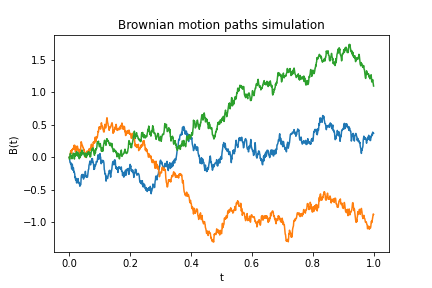
\includegraphics[scale = 0.6]{MS_Thesis_Template/figures/BM_paths.png}
    \caption{Simulation of Brownian motion paths.}
\label{bm_paths}    
\end{figure}
\begin{definition}[\textbf{Poisson Process}]
A stochastic process $\mathbf{N} = \{N_t ,t \geq 0\}$ defined on  $(\Omega,\mathcal{F},\mathbb{P})$ is called a Poisson process with rate $\lambda$ if it satisfies the following:\\
(1.) $N_0=0.$\\
(2.) For $0 \leq s < t$, $ N_{t} - N_s \stackrel{d}{=} Poiss(\lambda(t-s))$ i.e., for $k \in \mathbb{N}$ we have that,\\
\begin{equation}
    \mathbb{P}(N_t - N_s = k) = \frac{(\lambda(t-s))^{k} e^{-\lambda(t-s)}}{k!}.\\
\end{equation}
(3.) For $0<t_1<t_2<...<t_k$ we have that $N_{t_{1}},N_{t_{2}}-N_{t_{1}},...,N_{t_{k}}-N_{t_{k-1}}$ are independent.\\
\end{definition}
\textbf{Note:} For a Poisson process for small interval dt we have that:
\begin{equation}
  \mathbb{P}(N_{t+dt} - N_t = k) = \mathbb{P}(dN_t = k) =\left\{\begin{array}{lr}
        \lambda dt + o(dt), & \text{if } k = 1\\
        o(dt), & \text{if } k \geq 2\\
        1 - \lambda dt + o(dt) , &\text{if } k = 0
        \end{array}\right  
\label{p_inc}        
\end{equation}
Fig \ref{p_paths} shows simulation of some poisson process sample paths.

\begin{figure}[H]
    \centering
    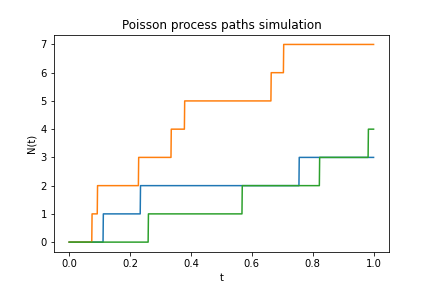
\includegraphics[scale = 0.6]{MS_Thesis_Template/figures/Poisson_simulation.png}
    \caption{Simulation of Poisson process paths with \lambda = 5.}
\label{p_paths}    
\end{figure}

\begin{definition}[\textbf{Filtration}]
A filtration on a $(\Omega , \mathcal{F}, \mathbb{P})$ is a non-decreasing family of sub sigma algebras of $\mathcal{F}$ denoted by $\{\mathcal{F}_t, t \in \mathcal{I}\}$ such that for $ s \leq t$ we have that $\mathcal{F}_s\subseteq \mathcal{F}_t \subseteq \mathcal{F}$.
\end{definition}

\begin{definition}[\textbf{Adapted Stochastic process}]
A stochastic process $\mathbf{X} = \{X_t ,t \in \mathcal{I}\}$ is said to be adapted to a filtration $\{\mathcal{F}_t, t \in \mathcal{I}\}$ if $X_t$ is $\mathcal{F}_t$-measurable for every $t \in \mathcal{I}$.
\end{definition}
\textbf{Note:} A stochastic process $\mathbf{X} = \{X_t ,t \in \mathcal{I}\}$ is always adapted to the filtration it generates denoted by $\{\mathcal{F}^{X}_t, t \in \mathcal{I}\}$ where $\mathcal{F}^{X}_t = \sigma(\{X_s :s \leq t \}).$

\begin{definition}[\textbf{Martingale process}]
A stochastic process $\mathbf{X} = \{X_t ,t \in \mathcal{I}\}$ is said to be a martingale with respect to a filtration $\{\mathcal{F}_t, t \in \mathcal{I}\}$ if the following holds:
\begin{enumerate}
    \item (\textbf{Adapted}) $X_t$ is $\mathcal{F}_t$-measurable for all $t \in \mathcal{I} $.
    \item (\textbf{Integrable}) $\E[|X_t|] < \infty.$
    \item (\textbf{Martingale property}) $\E[X_t | \mathcal{F}_{s}] = X_s$ for $s \leq t.$
\end{enumerate}
\end{definition}
\textbf{Note:} From the martingale property we have that $\E[X_t] = \E[\E[X_t | \mathcal{F}_{s}]] = \E[X_s] $. This implies that Martingale processes have constant expectation.







\section{A Primer on Option theory}
In this section we give an introduction to Option theory and some financial terminologies that are required for the project. The Theory in this section is covered from \cite{campolieti_2014} and \cite{papanicolaou_2019}.\\
A security is a financial instrument that has monetary value and which can be traded in Financial markets. Financial markets often make use of securities with stocks and
bonds as its common types. A derivative is a type of security whose value is derived from another underlying asset. An option contract is also a derivative such that the underlying asset in this case is stock.Options are of two types namely call and put options.We give the proper definition of an Option Contract. 

\begin{definition}A call(put) option is a contract that gives its holder
the right, but not the obligation, to buy(sell) a specific asset at a specified price(called the strike price) on or before a specific time(called the maturity time). 
\end{definition}
Options are further classified into two types namely European and American options with the former can be exercised only at the maturity time and the latter can be exercised on or before the maturity time. In this project we will only deal with European options.\\
Let $S_t$ be the price of a stock at time t. Consider a European option with the stock as its underlying with strike price denoted by $K$ and maturity time of the contract denoted by $T$. Then the call option payoff and put option payoff denoted by $\delta_{Call}$ and $\delta_{Put}$ respectively are given by,

$$\delta_{Call} = max(S_T-K,0)=(S_T-K)^+.$$ $$\delta_{Put}=max(K-S_T,0)=(K-S_T)^+.$$
Fig \ref{payoff} shows the payoff diagram for both put and call option with $K=50$.

\begin{figure}[H]
    \centering
    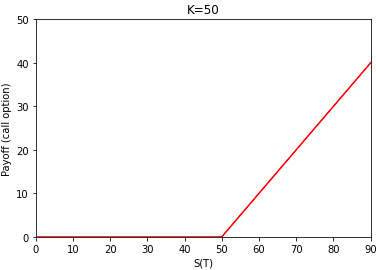
\includegraphics[scale = 2]{MS_Thesis_Template/figures/call.png}
    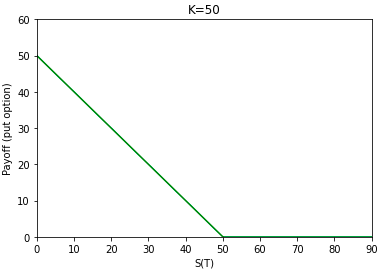
\includegraphics[scale =2]{MS_Thesis_Template/figures/put.png}
    
    
    \caption{Options pay off diagram. }
\label{payoff}    
\end{figure}
We now discuss the notion of moneyness for option. An option is said to be in the money when the option yields positive payoff (i.e., when $K < S_t$ for call option and $S_t < K$ for put option.).It is said to be out of the money when the option yields no payoff (i.e., when $K > S_t$ for call option and $S_t > K$ for put option.).It is said to be at the money when $S_t = K$ for both call and put option.\\
We now give an important relationship known as put-call parity that holds between the price of a European call and put option defined on a same underlying asset. Let $C$ and $P$ be the price of the European call and put option respectively.The put call parity is given by,\\
$$C + Ke^{-rT} = P + S_0. $$
Put-call parity relation is quite important as it can be used to know the price of a put option given that we know the price of a call option on the same underlying and vice versa. For a detailed proof of put-call parity the reader is encouraged to refer to $\cite{campolieti_2014}$.

\begin{definition}{(Definition 1.1.1 ,\cite{papanicolaou_2019})}An arbitrage opportunity is a trading opportunity that allows an investor to have a non zero probability of getting a profit and zero probability of getting a loss respectively given that his initial wealth was zero.
\end{definition}


\begin{theorem}{(Theorem 4.5,\cite{campolieti_2014})}
Under the assumption of absence of arbitrage followings are true :
\begin{equation}
\begin{aligned}
    (S_0-Ke^{-rT})^+ \leq C < S_0.\\
    (Ke^{-rT}-S_0)^+ \leq P < Ke^{-rT}.
\end{aligned}
\end{equation}
where $C$ and $P$ are the European Call and Put option price respectively.
\end{theorem}
For a proof of the above bounds please refer to \cite{campolieti_2014}.



\chapter{Stochastic Calculus and the Black Scholes Model}
In this chapter we will first cover some important properties of Brownian motion which then will be followed by rigorously covering Stochastic Calculus. At the end we will cover the Black Scholes model for option pricing. Theory in this chapter is mainly covered from \cite{mikosch_2011},\cite{shreve_2011}, \cite{resnick_1992} and \cite{oksendal_2013}.  

\section{Properties of Brownian Motion}
We now list out some of the important properties of Brownian Motion with a brief outline of proof of some of them.
\begin{enumerate}
    \item $\mathbf{B} = \{B_t ,t \geq 0\}$ is a \textbf{Gaussian process}\\
    \textbf{Proof:} We have to check that for $0\leq t_1<t_2<...<t_k$ the random vector $(B_{t_{1}},B_{t_{2}},...,B_{t_{k}})$ is multivariate gaussian.This can be checked by observing that for $c_i \in \mathbb{R}, 1 \leq i \leq k $ we have $c_{1}B_{t_{1}} + c_{2}B_{t_{2}}+...+c_{k}B_{t_{k}} = c_{k}(B_{t_{k}} - B_{t_{k-1}} ) + (c_{k}+c_{k-1})(B_{t_{k-1}}-B_{t_{k-2}})+...+(c_{k}+c_{k-1}+...+c_{1})B_{t_{1}}  $. The right hand side by the independent increments of $\mathbf{B}$ is normally distributed.\\ Now by Definition 3.1.1 it can be checked that $\mathbf{B}$ is a Gaussian process with mean zero and covariance given by,\\
    $$ Cov(B_s , B_t)  = s \wedge t.$$
    
    \item \textbf{Differential property:} For any $s > 0$, $\{B_{t+s} - B_{s},t \geq 0\}$ is a standard Brownian motion independent of $\{B(u),u\leq s\}$.
    
    \item \textbf{Scaling property:} For $c \geq 0$,$\{\sqrt{c}B(\frac{t}{c}), t \geq 0\}$ is a standard Brownian motion.
    
    \item \textbf{Symmetry property:} $\{-B_{t} ,t \geq 0\}$ is a standard Brownian motion.
    
    \item \textbf{Time inversion property:} Let $\{B^{1}(t) ,t \geq 0\}$ be a stochastic process defined as,
    $$B^1(t) =\left\{\begin{array}{lr}
        tB(\frac{1}{t}), & \text{if } t > 0\\
        0 & \text{if } t=0
        \end{array}\right $$
    then $\{B^{1}(t) ,t \geq 0\}$ is a standard Brownian motion.\\    
    \textbf{Proof:} We check each of the conditions of Definition 3.1.1.\\
    (\romannum{1}) Clearly, $B^1(0) = 0$.\\
    (\romannum{2}) For $0<s<t$, we check that
    $B^{1}(t) - B^{1}(s) \stackrel{d}{=} \mathcal{N}(0,t-s)$.\\ \begin{align*}
     B^{1}(t) - B^{1}(s) = (t-s)B\Big(\frac{1}{t}\Big) - s\Big(B\Big(\frac{1}{s}\Big) - B\Big(\frac{1}{t}\Big)\Big).   
    \end{align*}\\The right hand side is a linear combination of independent normal random variables and so $B^{1}(t) - B^{1}(s)$ is normally distributed. Now we have that,\\
    \begin{align*}
        E[B^{1}(t) - B^{1}(s)] &= E\Big[tB\Big(\frac{1}{t}\Big) - sB\Big(\frac{1}{s}\Big)\Big] = 0.\\
        Var[B^{1}(t) - B^{1}(s)] &= Var\Big[(t-s)B\Big(\frac{1}{t}\Big) - s(B\Big(\frac{1}{s}\Big) - B\Big(\frac{1}{t}\Big)\Big)\Big]. \\
        &= \frac{(t-s)^2}{t} + s^2\Big(\frac{1}{s} - \frac{1}{t}\Big).\\ 
        &= t-s.\\
    \end{align*}
    (\romannum{3}) We check the independent increment condition. Let $t_1 < t_2 < t_3$ then,\\
    \begin{align*}
        Var[B^1(t_3) - B^1(t_1)] &= t_3 - t_1.\\
        &= (t_3 - t_2) + (t_2 - t_1).\\ 
        &= Var[B^1(t_2) - B^1(t_1)] + Var[B^1(t_3) - B^1(t_2)].
    \end{align*}
    This implies that the increments $B^1(t_2) - B^1(t_1)$ and $B^1(t_3) - B^1(t_2)$ are uncorrelated and since they are jointly gaussian as well, therefore the increments are independent.\\
    (\romannum{4}) Clearly, $B^1(t) = tB(\frac{1}{t})$ is continuous for $\forall t > 0$. For the proof of continuity at t=0 refer to \cite{resnick_1992}.
    \item The sample paths of Brownian motion are \textbf{nowhere differentiable}.\\
    \textbf{Proof:} For the detailed proof refer to \cite{resnick_1992}.\\ Nowhere differentiability can also be shown by using distributional arguements by observing that $\frac{B_{t+h}-B_t}{h} \stackrel{d}{=} \frac{\mathcal{N}(0,h)}{h} \stackrel{d}{=} \mathcal{N}(0,\frac{1}{h}) $ which implies that the slope of the sample paths has infinite variance almost everywhere, therefore the sample paths are nowhere differentiable.
    \item \textbf{Finite Quadratic variation:} Let $\pi := \{0=t_0<t_1<...<t_{n-1}<t_n=T\}$ be a partition of $[0,T]$ such that $|\pi| = max_{1 \leq i \leq n} (t_i - t_{i-1})\xrightarrow{n\longrightarrow \infty} 0 $ .\\Then we have the following:
    \begin{equation}
       \sum_{i=1}^{n} (B_{t_i} - B_{t_{i-1}})^{2} \xrightarrow[|\pi|\longrightarrow 0]{L^{2}} T. 
    \end{equation}
    \textbf{Proof}: Denote the quadratic variation over $[0,T]$ by $[\mathbf{B},\mathbf{B}](T)$. Then we have that,\\
    \begin{align*}
       \E[\sum_{i=1}^{n} (B_{t_i} - B_{t_{i-1}})^{2}] = \sum_{i=1}^{n} E[(B_{t_i} - B_{t_{i-1}})^{2}] &= \sum_{i=1}^{n}(t_i - t_{i-1})\\
       &= T.\\
       \Var[\sum_{i=1}^{n} (B_{t_i} - B_{t_{i-1}})^{2}] = \sum_{i=1}^{n} \Var[(B_{t_i} - B_{t_{i-1}})^{2}]
       &=2\sum_{i=1}^{n}(t_i - t_{i-1})^{2}\\
       & \leq 2|\pi|T \xrightarrow{|\pi|\longrightarrow 0} 0.
    \end{align*}
    
    Thus $ \sum_{i=1}^{n} (B_{t_i} - B_{t_{i-1}})^{2} \xrightarrow[|\pi|\longrightarrow 0]{L^{2}} \E[ \sum_{i=1}^{n} (B_{t_i} - B_{t_{i-1}})^{2}]=T$
    and $[\mathbf{B},\mathbf{B}](T) = T$.\\
    \item \textbf{Unbounded first variation:} Let $\pi$ be the same partition of $[0,T]$ as defined in property (7). Then the first variation of Brownian motion is infinite a.s. i.e.,\\
    $$\sup_{\pi} \sum_{i=1}^{n} |B_{t_i} - B_{t_{i-1}}| = \infty \hspace{0.3cm}a.s.$$
    \textbf{Proof:} Let $T=1$ and $\Delta_i B=B_{t_i} - B_{t_{i-1}}$. Suppose $\sup_{\pi} \sum_{i=1}^{n} |B_{t_i} - B_{t_{i-1}}| < \infty$.\\Then,
    \begin{equation}
        \begin{aligned}
           \sum_{i=1}^{n} (\Delta_i B)^2 \leq \max\limits_{i=1,...,n}|(\Delta_i B)| \sum_{i=1}^{n} |(\Delta_i B)| & \leq \max\limits_{i=1,...,n} |(\Delta_i B)| \sup_{\pi}\sum_{i=1}^{n} |(\Delta_i B)|\\
           & \xrightarrow{|\pi|\longrightarrow 0 } 0 \hspace{0.5cm}a.s.
        \end{aligned}
        \label{uniform_cont}
    \end{equation}
    \ref{uniform_cont} holds because $\max\limits_{i=1,...,n}|(\Delta_i B)|\xrightarrow{|\pi|\longrightarrow 0 } 0 $ as $B_t$ is uniformly continuous a.s.\\ From property (7) we have that,\\
    \begin{align*}
       \sum_{i=1}^{n} (\Delta_i B)^2 \xrightarrow[|\pi|\longrightarrow 0]{L^{2}} 1 &\Longrightarrow \sum_{i=1}^{n} (\Delta_i B)^2 \xrightarrow[|\pi|\longrightarrow 0]{\mathbb{P}} 1\\
       & \Longrightarrow \sum_{i=1}^{n_k} (\Delta_i B)^2 \xrightarrow[|\pi|\longrightarrow 0]{a.s.} 1.
    \end{align*}
    \hspace{7cm}(along some subsequence $n_k$)\\
    Then we must have that \ref{uniform_cont} happens only on a measure zero set.\\
    $\Longrightarrow \mathbb{P}(\{\sup_{\pi} \sum_{i=1}^{n} |B_{t_i} - B_{t_{i-1}}| = \infty\}) = 1$ and we are done.
    \item \textbf{Martingale property:} $\{B_t,t \geq 0 \}$ is a martingale process w.r.t. $\{\mathcal{F}_t,t \geq 0 \}$ where $\mathcal{F}_t = \sigma(B_s,s \leq t)$.\\
    \textbf{Proof:} Adaptibility of Brownian motion process is clear. Further from Cauchy-Schwarz inequality we have that $E[|B_t|] \leq \sqrt{E[B_{t} ^2]} = \sqrt{t} < \infty$.\\We now prove the martingale property let $s<t$,\\
    \begin{align*}
        \E[B_t | \mathcal{F}_{s}] &= \E[(B_t - B_s)| \mathcal{F}_{s}] + \E[B_s | \mathcal{F}_{s}]. \\
        &=\E[B_t - B_s] + B_s \;\; \mbox{(As $B_t - B_s$ is independent of $\mathcal{F}_{s}$ and $B_s \in \mathcal{F}_{s}$ ).}\\
        &= B_s.
    \end{align*}
    Further it can also be shown that $\{B_{t} ^2 -t,t \geq 0 \} $ and $\{\exp(cB_t - \frac{1}{2}c^2 t),t \geq 0 \}$ are both also martingales w.r.t. $\{\mathcal{F}_t,t \geq 0 \}$. 
    
    
    
    
\end{enumerate}
\section{Stochastic Calculus}
We first give a proper motivation for introducing Stochastic Calculus. We are particularly interested in integrals of the form  $\int_{0}^{T} f(s) \,dB_s(\omega)\ $ and $\int_{0}^{T} B_s(\omega) \,dB_s(\omega)\ $ where $f$ is a deterministic function or a function of stochastic process which is adapted to the brownian motion filtration. In ordinary calculus we deal with these integrals by the Riemann-Stieljes approach. We first discuss the major problem that arises if we proceed with this approach. For simplicity we suppose T = 1.
\begin{definition}
For $p > 0$, the $p$-variation of a function $f:\mathbb{R} \rightarrow \mathbb{R}$ on $[0,1]$ is defined as:
\begin{equation}
    V^{p}(f) = \sup_{\pi}\sum_{i=1}^{n} |f(t_i) - f(t_{i-1})|^{p}.
\end{equation}
where the supremum varies over the partitions $\pi$ of $[0,1]$. $f$ is said to be a function  of bounded p-variation on $[0,1]$ if $V^{p}(f) < \infty$.

\end{definition}
The following theorem provides sufficient condition under which the Riemann-Stieljes integral $\int_{0}^{1}f(x)dg(x)$} exists for some functions $f$ and $g$.

\begin{theorem}
The Riemann-Stieljes integral $\int_{0}^{1}f(x)dg(x)$} exists provided the following are satisfied:
\begin{enumerate}
    \item $f$ and $g$ do not have discontinuities at the same points on $[0,1]$.
    \item $V^{p}(f) < \infty$ and $V^{q}(g) < \infty$ for some $p,q > 0$ such that $\frac{1}{p} + \frac{1}{q} > 1$.
\end{enumerate}
\end{theorem}

Further for Brownian motion sample paths it is known that $V^{p}(B_{t}) < \infty$ for $p>2$ and $V^{p}(B_{t}) = \infty$ for p \leq 2.\par
Since $V^{1}(B_{t}) = \infty$ we will have that $\int_{0}^{1} f(s) \,dB_s(\omega)\ $ exists in the Riemann-Stieljes sense provided $V^{1}(f_{t}) < \infty$ i.e., we are forced to consider only functions of bounded first variation and further $\int_{0}^{1} B_s(\omega) \,dB_s(\omega)\ $ does not exist in the Riemann-Stieljes sense.To deal with these problems the theory of Stochastic calculus is introduced. 
\subsection{Itô Integral}
Let $\mathcal{L}_2$ be the space of all stochastic processes $\mathbf{X} = \{X_t ,t \geq 0\}$ adapted to the Brownian motion filtration s.t. $E[\int_{0}^{T} X_{s}^{2}ds] < \infty$ and the Riemann integral $\int_{0}^{T}X_{s}ds$ exists a.s., $\forall T>0$. We first define the Itô Integral for simple processes in this space of stochastic processes and then extend the definition of the Itô Integral for any general process in this space.
\begin{definition}
A stochastic process $\mathbf{X} \in \mathcal{L}_{2}$ is called simple if there exists a countable partition $\{t_n\}_{n \in \mathbb{N} \cup \{0\}$ s.t. $X_{t}(\omega)=X_{t_{j}}(\omega)$, $\forall t \in [t_j,t_{j+1}) $ and $\forall \omega \in \Omega$.\\
The Itô Integral denoted $I_{t}(\mathbf{X})$ for such simple processes for $t_{n}\leq t < t_{n+1}$ is given by,\\
\begin{equation}
    I_{t}(\mathbf{X}) = \int_{0}^{t}X_{s}dB_{s} = \sum_{j=0}^{n-1}X_{t_{j}}(B_{t_{j-1}} - B_{t_{j} }) + X_{t_{n}}(B_{t} - B_{t_{n}}).
\end{equation}
\end{definition}
The following important properties holds for the Itô Integral of simple processes.
\begin{theorem}
The Itô Integral for simple processes satisfies the following:
\begin{enumerate}
    \item(\textbf{Linearity}) $I_{t}(a\mathbf{X} + b\mathbf{Y}) = aI_{t}(\mathbf{X})+bI_{t}(\mathbf{Y}).$
    \item(\textbf{Itô Isometry}) $E[(I_{t}(\mathbf{X}))^{2}] = E[\int_{0}^{t}X_{s}^{2}ds].$
    \item$\{I_{t}(\mathbf{X}) , t \geq 0\}$ is a martingale w.r.t. Brownian motion filtration.
    \item$I_{t}(\mathbf{X})$ has continuous sample paths.
    \item(\textbf{Quadratic variation}) $[I,I](t) =\int_{0}^{t}X_{s}^{2}ds $.
\end{enumerate}
\end{theorem}
Now given any general stochastic process in $\mathcal{L}_{2}$ it can be shown that it can be approximated by a sequence of simple processes in the sense defined in the below theorem.
\begin{theorem}
Given any general stochastic process $\mathbf{X} \in \mathcal{L}_{2}$, $\exists$ a sequence of simple processes $\mathbf{X}^{n} \in \mathcal{L}_{2} $ such that, 
\begin{equation}
    \lim_{n \to \infty}E\Big[\int_{0}^{T}(X_{s}^{n}-X_{s})^{2}ds\Big] = 0.
\end{equation}
\end{theorem}
For the detailed proof of above theorem refer to \cite{resnick_1992}. 
\begin{theorem}
Let $\mathbf{X}^{n} \in \mathcal{L}_{2} $ be a simple process that satisfies the above theorem.Then there exists a stochastic process $Z_t$ satisfying,
\begin{equation}
    \lim_{n \rightarrow \infty} E\left[(Z_t-I_t(X^n))^2\right]=0 ,\forall t \in [0,T].
\end{equation}
The stochastic process $Z_t$ is unique in the sense that if $\Hat{{X}^{n}} $ is another simple process satisfying the above theorem and let $\Hat{Z_t}$ be its limit in the above sense then,
\begin{equation}
  \mathbb{P}(\Hat{Z_t} = Z_t , \forall t \in [0,T]) = 1.
\end{equation}  

\end{theorem}
\begin{theorem}
Let $\mathbf{X} \in \mathcal{L}_{2} $ be a general stochastic process then its Itô Integral $I_t(X)$ is defined as the unique stochastic process $Z_t$ defined in the above theorem. 
\end{theorem}
Thus to compute $I_t(X)$ for general process $\mathbf{X} \in \mathcal{L}_{2} $ we first need to obtain a sequence of simple processes in $\mathcal{L}_{2}$ satisfying theorem 3.2.3 and then $I_t(X)$ is given by the limit of the Itô Integral of those simple processes in the mean square sense.

\begin{theorem}
The Itô Integral for any general process in $\mathcal{L}_{2}$ satisfies the following:
\begin{enumerate}
    \item(\textbf{Linearity}) $I_{t}(a\mathbf{X} + b\mathbf{Y}) = aI_{t}(\mathbf{X})+bI_{t}(\mathbf{Y})$.
    \item(\textbf{Itô Isometry}) $E[(I_{t}(\mathbf{X}))^{2}] = E[\int_{0}^{t}X_{s}^{2}ds]$.
    \item$\{I_{t}(\mathbf{X}) , t \geq 0\}$ is a martingale w.r.t. Brownian motion filtration.
    \item$I_{t}(\mathbf{X})$ has continuous sample paths. 
    \item(\textbf{Quadratic variation}) $[I,I](t) =\int_{0}^{t}X_{s}^{2}ds $.
\end{enumerate}
\end{theorem}

\begin{example}
We will now compute $I_{T}(\mathbf{\mathbf{B}})=\int_{0}^{T} B_t \,dB_t\ $.
\end{example}

Consider the sequence of partitions $\pi_{n}:=\{0=t_0<t_{1}<...<t_{n}=T\}$ such that $|\pi_{n}| \xrightarrow[]{n \longrightarrow \infty} 0 $. Now consider the following process $\mathbf{B}^{n} $ where
$B_{t}^{n} = B_{t_{j}} ,\forall t\in [t_{j},{t_{j+1}})$. Clearly $\mathbf{B}^{n} $ is a sequence of simple processes such that,\\
\begin{aligned}
E\Big[\int_{0}^{T} (B_{t}-B_{t}^{n})^{2}dt\Big]=E\Big[\sum_{j=0}^{n-1}\int_{t_j}^{t_{j+1}} (B_{t}-B_{t_{j}})^{2}dt\Big]
 &=\sum_{j=0}^{n-1}\int_{t_j}^{t_{j+1}}E[ (B_{t}-B_{t_{j}})^{2}]dt\\
 &=\sum_{j=0}^{n-1}\frac{(t_{j+1}-t_{j})^{2}}{2}\\
 &\leq \frac{1}{2}|\pi_{n}|T \xrightarrow[]{n \to \infty} 0.
\end{aligned}\\
Thus the sequence of simple processes $\mathbf{B}^{n} $ satisfies theorem 3.2.3 and so we need to compute the limit of $ I_{T}(\mathbf{\mathbf{B}^{n}})$ in mean square sense.\par
\textbf{Note:} $ I_{T}(\mathbf{\mathbf{B}^{n}}) = \sum_{j=0}^{n-1}B_{t_j}(B_{t_{j+1}}-B_{t_{j}})$. Then we have that,\par
\begin{aligned}
 B^{2}(T) - B^{2}(0) &=\sum_{j=0}^{n-1} (B_{t_{j+1}}^{2}-B_{t_{j}}^{2})\\ 
 \Longrightarrow B^{2}(T)&= \sum_{j=0}^{n-1}(B_{t_{j+1}}-B_{t_{j}})^{2} +2\sum_{j=0}^{n-1}B_{t_j}(B_{t_{j+1}}-B_{t_{j}})\\
 \Longrightarrow I_{T}(\mathbf{\mathbf{B}^{n}})& = \frac{1}{2}B^{2}(T)- \frac{1}{2}\sum_{j=0}^{n-1}(B_{t_{j+1}}-B_{t_{j}})^{2}\\
 &\xrightarrow[n \longrightarrow \infty]{L^{2}} \frac{1}{2}B^{2}(T) - \frac{T}{2}.
\end{aligned}

Thus $I_{T}(\mathbf{B})= \int_{0}^{T} B_t \,dB_t\ = \frac{1}{2}B^{2}(T) - \frac{T}{2}$.\\
We observe that for the Itô Integral the convention is that the simple processes are evaluated at the left end point of the partitions. One important property about the Stochastic Integral is that the integral actually depends on where the simple processes are evaluated as opposed to the Riemann-Stieljes approach where the choice of evaluation point of the integrand doesn't matter provided that the Riemann-Stieljes integral exists.\par 
To demonstrate this consider again example 3.2.1 with the following simple processes $\mathbf{B}^{n} $ where
$B_{t}^{n} = B_{t_{j}^{*}} ,\forall t\in [t_{j},{t_{j+1}})$ where $t_{j}^{*}= \frac{t_{j+1}+t_{j}}{2}$. Then it can be shown that,\par
$$\sum_{j=0}^{n-1}B_{t_{j}^{*}}(B_{t_{j+1}}-B_{t_{j}}) \xrightarrow[n \longrightarrow \infty]{L^{2}} \frac{1}{2}B^{2}(T).$$
The stochastic integral where the simple processes are evaluated at mid point is known as the \textbf{Stratonovich Integral} denoted by $\int_{0}^{T} B_to\,dB_t\ = \frac{1}{2}B^{2}(T)$.

\subsection{Itô formula}
Itô formula is a analogous chain rule of differentiation for stochastic calculus. If $f$ is a differentiable function then from the ordinary chain rule of calculus the differential $df(B_t)=f^{'}(B_t)dB_t$ is no longer valid due to non-differentiablity of Brownian motion sample paths and it has to be corrected by an additional term due to non-zero quadratic variation of Brownian motion sample paths which is given by the Itô formula. We first give the definition of Itô processes.
\begin{definition}
A stochastic process $\mathbf{X}$ is called Itô process if it can be written as:
 \begin{equation}
     X_t = X_0 +\int_{0}^{t}a(s,X_s)ds + \int_{0}^{t}b(s,X_s)dB_s.
 \end{equation}

where both $a(s,X_s)$ and $b(s,X_s)$ are adapted to Brownian motion filtration. It is assumed here that the first integral exists in the Riemannian sense and second integral in the Itô sense.
\end{definition}\par
We observe that Brownian motion is also a type of Itô process for the case when $a(s,X_s)=0$ and $b(s,X_s) = 1$ in 3.8.It can be checked that the quadratic variation of Itô process is given by $[\mathbf{X},\mathbf{X}](T)=\int_{0}^{T}(b(s,X_s))^{2}ds$. For computational convenience we often write 3.8 in the following differential form:
\begin{equation}
    dX_t = a(t,X_t)dt + b(t,X_t)dB_t.
\end{equation}
Now using $(dB_t)^2 = dt$ and $(dt)^2 = dB_t~dt = 0$ (in mean square sense) we will have,
$$(dX_t)^2 = \Big(a(t,X_t) dt + b(t,X_t) dB_t\Big)\Big(a(t,X_t) dt + b(t,X_t) dB_t\Big) = (b(t,X_t))^{2} dt.$$


\begin{theorem}{\textbf{Itô Formula for Ito Process}}
Let $X_t$ be an Ito process as defined in 3.8. Let $f(t,x)$ be a function whose partial derivatives $f_1(t,x),f_2(t,x)$ and $f_{22}(t,x)$ exists and are continuous. Then we have:
\begin{equation}
    f(t,X_t) - f(X_0,0) = \int_{0}^{t}f_1(s,X_s)ds + \int_{0}^{t}f_2(s,X_s)dX_s  + \frac{1}{2} \int_{0}^{t}f_{22}(s,X_s)(dX_s)^2.
\end{equation}
 
\end{theorem}
We write 3.10 in the following differential form for computational purpose:
\begin{equation}
    df(t,X_t) = f_1(t,X_t) dt + f_2(t,X_t) dX_t + \frac{1}{2} f_{22}(t,X_t) (dX_t)^2. 
\end{equation}
\begin{equation}
    df(t,X_t) = \Big[f_1 (t,X_t) +a(t,X_t) f_2(t,X_t) +  \frac{1}{2} b(t,X_t)^2 f_{22}(t,X_t)\Big] dt  + b(t,X_t) f_2(t,X_t) dB_t. 
\end{equation}
Itô Formula is used to solve Itô stochastic differential equations of the form 3.9. We illustrate it through an example of stochastic differential equation.
\begin{example}[Geometric Brownian Motion]
The S.D.E. of Geometric Brownian Motion is obtained by considering $a(t,X_t) = \mu X_{t}$ and $b(t,X_t) = \sigma X_{t}$ in 3.9 where $\mu$ and $\sigma > 0$  are constants.\par
\begin{equation}
    dX_t = \mu X_{t}dt + \sigma X_{t}dB_t. 
\label{gbm_sde}    
\end{equation}
We consider the following function $f(t,x) = \log(x)$ for applying Itô's Formula. Now $f_{1}(t,x)=0$,$f_{2}(t,x)=\frac{1}{x}$ and $f_{22}(t,x)=-\frac{1}{x^{2}}$. We have that all the required partial derivatives exist and are continuous then by 3.12 we have, \par
\begin{equation}
\begin{align*}
    &d\log(X_t) = \Big[\mu X_t  \frac{1}{X_t} - \frac{1}{2} (\sigma X_t)^2 \frac{1}{(X_t)^{2}}\Big]dt + \sigma X_t \frac{1}{X_t} dB_t\\
    &d\log(X_t) = \Big[\mu - \frac{1}{2} \sigma^2\Big]dt + \sigma dB_t\\
    &\log(\frac{X_t}{X_0}) = \int_{0}^{t}\Big(\mu - \frac{1}{2}\sigma^{2}\Big)ds + \int_{0}^{t}\sigma dB_s\\
    \Longrightarrow &X_t = X_0 e^{\sigma B_t + (\mu - \frac{1}{2}\sigma^{2})t}.\\
\end{align*}
\label{gbm_sol}
\end{equation}
The stochastic process $X_t$ in \ref{gbm_sol} is the solution of the S.D.E. \ref{gbm_sde} known as Geometric Brownian Motion and it is an important stochastic process for modelling stock prices.


\end{example}
Fig \ref{gbm_paths} shows simulation of some paths of geometric brownian motion.

\begin{figure}[H]
    \centering
    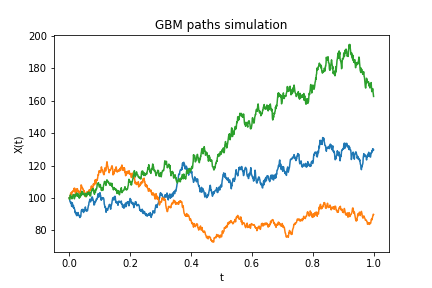
\includegraphics[scale = 0.6]{MS_Thesis_Template/figures/GBM_paths.png}
    \caption{Simulation of GBM paths with $S_0 =100,\mu = 0.2$ and $\sigma = 0.3.$}
\label{gbm_paths}    
\end{figure}


\section{Black Scholes Model for Option pricing}
We have covered the theory required to understand the mathematical framework of continuous time option pricing model. In this section we cover the benchmark option pricing model i.e., the Black Scholes Model. The following assumptions are to be made for the model:\\
(1.) We only consider European options.\\
(2.) We assume that there exists no arbitrage opportunities in the market.\\ 
(3.) We also assume that the stock pays no dividend and there are no transaction costs.\\
(4.) The Stock price follows lognormal distribution\footnote{This assumption is due to the efficient market hypothesis and an application of the Central limit theorem. For more detail refer to \cite{rosenkrantz_2009}} i.e., the log-returns are normally distributed.\\
(5.) The risk free interest rate $r$ and volatility of asset $\sigma$ are known and they are constant throughout the option's life.\\
We also have in our model that the risk free bank account $\beta_t$ evolves as :\\
\begin{equation}
    d\beta_t = r\beta_t dt.
\end{equation}
We also assume that stock price process $S_t$ evolves according to the geometric brownian motion:\\
\begin{equation}
    dS_t = \mu S_{t}dt + \sigma S_{t}dB_t.
\end{equation}
Let $C(t,S_t)$ be price of call option at time $t$ with strike price $K$ and maturity time $T$.We assume that all the partial derivatives of $C(t,S_t)$ required for the Itô Formula exist and are continuous. We will first derive the famous Black Scholes P.D.E. by using a replicating portfolio arguement.We consider a portfolio of the risk free bank account and the stock with $a_t$ (amount of shares in stock) and $b_t$(amount of shares in bank) such that both the stochastic process $a_t$ and $b_t$ are adapted to $\mathcal{F}_t, \forall t \in [0,T]$ where $\mathcal{F}_t = \sigma(B_s,s \leq t)$.Let $V(t,S_t)$ denote the value of the portfolio at time t then,\\
\begin{equation}
    V_t = a_{t}S_{t} + b_t\beta_{t}.
\end{equation}
Further we assume that the portfolio is self-financing i.e., the portfolio value evolves only due to the changes in the value of the stock and bank respectively and we do not inject any external money or take out any money from the portfolio during the process. Mathematically the self-financing condition is given by:\\
\begin{equation}
   dV_t = d(a_{t}S_{t} + b_t\beta_{t}) = a_{t}dS_{t} + b_td\beta_{t}. 
\end{equation}
Now for the replication arguement we want the portfolio to match the price of the call option at maturity i.e., $V(T,S_T) = C(T,S_T) = (S_T-K)^{+}$. Note that under this condition we must have $V_t=C(t,S_t) ,\forall t \in [0,T]$ due to no-arbitrage assumption. Indeed if we have $V(t,S_t) < C(t,S_t) $ for any $t \in [0,T]$ then one can sell the call option and buy the portfolio at time t. This strategy is an arbitrage opportunity as it will yield a profit of \Big($C(t,S_t) - V(t,S_t)$\Big) because at maturity we have that $C(T,S_T) = V(T,S_T)$ i.e., the call option payoff that has to be paid will be covered by the bought replicating portfolio at maturity. Similarly the other case $V(t,S_t) > C(t,S_t) $ will also result in arbitrage opportunity.\\
Now by the Itô formula we have that,\\
\begin{equation}
    dC_t = \Big[C_{1}(t,S_t) + \mu C_{2}(t,S_t) S_t + \frac{1}{2} \sigma^{2} S_t^{2} C_{22}(t,S_t)\Big]dt + \sigma C_2(t,S_t)S_t dB_t.
\end{equation}
We also have from 3.15 and 3.16,\\
$$dV_t = a_{t}dS_{t} + r b_t \beta_t dt = a_t\Big[\mu S_{t}dt + \sigma S_{t}dB_t\Big] + r \beta_t \Big(\frac{V_t - a_t S_t}{\beta_t}\Big) dt$$

\hspace{5.7cm}$= \Big[\mu a_t S_t + r(V_t - a_t S_t)\Big]dt + \sigma a_t S_t dB_t.$\\
We have that $dV_t = dC_t, \forall t \in [0,T] $. Equating the $dB_t$ coefficient gives,\\
\begin{equation}
    a_t = \frac{\partial C(t,S_t)}{\partial S_t}.
\end{equation}
Equating the drift terms and from 3.20 we get,\\
\begin{equation}
\frac{\partial C(t,S_t)}{\partial S_t} + \frac{(\sigma S_{t})^{2}}{2} \frac{\partial^{2} C(t,S_t)}{\partial S_{t}^{2}}+rS_{t}\frac{\partial C(t,S_t)}{\partial S_t} - rC(t,S_t) = 0.
\end{equation}
This is the famous Black scholes P.D.E. for European call options with the boundary conditions $C(t,0) = 0,$ $C(T,S_T) = (S_T - K)^{+}$ and $ C(t,S_t)\xrightarrow[]{S_t \longrightarrow \infty} S_t$. The Black Scholes option pricing formula can be obtained from the above P.D.E. by transforming it into a heat equation and using Fourier transform technique to solve it. In this project the Black Scholes formula will be derived using the Equivalent Martingale Measure which is covered in next section.
\subsection{Deriving the Black Scholes formula by Equivalent martingale measure technique}
In this section we will derive the Black Scholes formula by the Equivalent martingale measure technique. The idea of the proof is to change the probability measure $\mathbb{P}$ to another equivalent measure $\mathbb{Q}$ such that under $\mathbb{Q}$ we have the following:\\
(1.)$\{\widetilde{B_{t}} = B_{t} + ct ,0 \leq t \leq\ T \}$(Brownian motion with drift) becomes a standard Brownian motion under $\mathbb{Q}$.\\
(2.) $\{e^{-rt}S_t ,0 \leq t \leq\ T\}$ and $\{e^{-rt}V_t,0 \leq t \leq\ T \}$ are martingales under $\mathbb{Q}$.\\
An Equivalent Martingale Measure(E.M.M.) is an equivalent measure to $\mathbb{P}$ such that under it some stochastic process becomes a martingale. Girsanov's theorem is an important result which will give us the required equivalent measure $\mathbb{Q}$ and once we have shown point (2.) then this new measure $\mathbb{Q}$ will become the required E.M.M.
\begin{theorem}[Girsanov's Theorem]
Suppose $\Theta(t),\;0\leq t \leq T$ be an adapted process to Brownian motion filtration. Define:
$$
Z(t) = e^{-\int_{0}^{t}\Theta(u)dB_u - \frac{1}{2}\int_{0}^{t}\Theta^2(u)du}.
$$
$$
\tilde{B}_t = B_t + \int_{0}^{t}\Theta(u)du.
$$
Let $Z = Z(T)$, we define,
$$
\mathbb{Q}(A) = \int_A Z d\mathbb{P}(\omega),\;\;A\in\mathcal{F}.
$$ 
Then,\\
\begin{enumerate}
    \item $\mathbb{E}_\mathbb{P}[Z] = 1$ and $\mathbb{Q}$ is an equivalent probability measure to $\mathbb{P}.$
    \item $\tilde{B}_t$ is a standard Brownian motion under $\mathbb{Q}$.
\end{enumerate} 
\end{theorem}

In our case we want $\widetilde{B_{t}} = B_{t} + ct$ to be a standard Brownian motion where $c = \frac{\mu-r}{\sigma}$. Let $Z = e^{-cB_T - \frac{1}{2}c^2T}$ and define,\\
\begin{equation}
\mathbb{Q}(A) = \int_A Z(\omega) d\mathbb{P}(\omega),\;\;A\in\mathcal{F}.
\end{equation}
Then by Girsanov's theorem it follows that $\mathbb{Q}$ is the required equivalent probability measure such that under it $\widetilde{B_{t}}$ becomes a standard Brownian motion.\\
\textbf{Note:} Under $\mathbb{P}$ the stock price process is given by,\\
\begin{equation}
    S_t=S_{0}e^{\sigma B_{t}+(\mu-\frac{\sigma^{2}}{2})t}.
\end{equation}
Under $\mathbb{Q}$ the stock price process becomes,\\
\begin{equation}
    S_t = S_0 e^{\sigma \widetilde{ B_{t}}+(r-\frac{\sigma^{2}}{2})t}
\end{equation}
$$\implies E_{\mathbb{Q}}[S_t] = S_0 E_{\mathbb{Q}}[e^{\sigma \widetilde{ B_{t}}+(r-\frac{\sigma^{2}}{2})t}] = S_0 e^{rt}.$$
Therefore under this measure $\mathbb{Q}$, the stock on an average behaves as the risk free bank account and that is why this Equivalent Martingale Measure is also known as the Risk Neutral Measure.\\
Now we will prove that $\{e^{-rt}S_t ,0 \leq t \leq\ T\}$ is martingale under $\mathbb{Q}$. Let  $\widetilde{S_t} = e^{-rt}S_{t}$ and consider $f(t,x) = e^{-rt} x$ we have that,\\
$$f_{1}(t,x) = -r e^{-rt} x , f_{2}(t,x) = e^{-rt}, f_{22}(t,x) = 0. $$
Now apply the Itô Formula 3.11 for $\widetilde{S_t}$,\\
\begin{align*}
    d\widetilde{S_t}& = -re^{-rt}S_tdt + e^{-rt}dS_{t}\\
    &=\Big[-r e^{-rt} S_t + \mu S_t e^{-rt}\Big]dt + \sigma S_t e^{-rt} dB_t\\
    &=\widetilde{S_t}\Big[(\mu - r) dt + \sigma dB_t\Big]\\
    &=\sigma \widetilde{S_t} d\widetilde{B_t}.\\ 
    \implies& \widetilde{S_t} - \widetilde{S_0} = \int_{0}^{t}\sigma \widetilde{S}_ud\widetilde{B_u}.\\
\end{align*}

The right hand side is an Itô integral under the measure
$\mathbb{Q}$ and which by theorem 3.2.6(3.) we know that it is a martingale. Therefore $\widetilde{S_t} = e^{-rt}S_{t}$ is a martingale process under $\mathbb{Q}$.\\
Now we will prove that $\{e^{-rt}V_t ,0 \leq t \leq\ T\}$ is martingale under $\mathbb{Q}$. Let $\widetilde{V_t} = e^{-rt}V_{t}$ now again apply the Itô's Formula for $\widetilde{V_t}$ ,\\
\begin{align*}
   d\widetilde{V_t} & = -re^{-rt}V_tdt + e^{-rt}dV_{t}\\
                    & =e^{-rt}[-r V_t dt + a_t dS_t + b_t d\beta_t]\\
                    & =e^{-rt}[-r a_t S_t dt + \mu a_t S_t dt + \sigma a_t S_t dB_t]\\
                    & =a_t \widetilde{S_t} [(\mu - r) dt + \sigma dB_t]\\
                    & = \sigma a_t \widetilde{S_t} \widetilde{dB_t}.\\
                    \implies & \widetilde{V_t} - \widetilde{V_0} = \int_{0}^{t}\sigma a_u \widetilde{S}_ud\widetilde{B_u}. \\
\end{align*}

The right hand side is a martingale under $\mathbb{Q}$ and therefore $\widetilde{V_t} = e^{-rt}V_t$ is a martingale under $\mathbb{Q}$. Now by martingale property for $t \in [0,T]$ we will have that,
\begin{equation}
e^{-rt} V_{t} = E_{\mathbb{Q}}[e^{-rT}V_{T}|\mathcal{F}_{t}] 
\end{equation}

\begin{equation}
    V_{t} = E_{\mathbb{Q}}[e^{-r(T-t)}V_{T}|\mathcal{F}_{t}].
\end{equation}

We have that $V_t = C_t , \forall t \in [0,T]$ and $V_T = (S_T - K)^{+}$ this gives, 
\begin{equation}
C(t,S_{t}) =E_{\mathbb{Q}}[e^{-r(T-t)} (S_{T}-K)^{+}|\mathcal{F}_{t}].
\end{equation}
For $t=0$ the above becomes,\\
\begin{align*}
  C(0,S_{0}) & =E_{\mathbb{Q}}[e^{-rT} (S_{T}-K)^{+}]\\            & =E_{\mathbb{Q}}[e^{-rT} (S_{T}-K) \mathbb{I}_{\{S_{T} > K\}}]\\
             & =E_{\mathbb{Q}}[e^{-rT} S_{T} \mathbb{I}_{\{S_{T} > K\}}] - K e^{-rt} E_{\mathbb{Q}} [\mathbb{I}_{\{S_{T} > K\}}]\\
             & =E_{\mathbb{Q}}[e^{-rT} S_{T} \mathbb{I}_{\{S_{T} > K\}}] - K e^{-rt} \mathbb{Q}(\{S_{T} > K\}).
\end{align*}
\textbf{Note:} $S_T =S_0 e^{\sigma \widetilde{ B_{T}}+(r-\frac{\sigma^{2}}{2})T} \stackrel{d}{=} S_0 e^{\sigma \sqrt{T} Z+(r-\frac{\sigma^{2}}{2})T} $ where $Z$ is the standard normal random variable. Now,\\
\begin{align*}
  S_T>K & \iff S_0 e^{(r -\frac{1}{2}\sigma^2)T + \sigma \sqrt{T}Z} > K  \\
  & \iff Z> \frac{\log(K/S_0)-(r-\sigma^2/2)T}{\sigma\sqrt{T}} \\
  & ~~~~~~~~~~~= \sigma\sqrt{T}-d_1,
\end{align*}
where $$ d_1 = \frac{log(\frac{S_{0}}{K}) + (r+\frac{\sigma^{2}}{2})T}{\sigma \sqrt{T}}.$$

\begin{align*}
    E_{\mathbb{Q}}[e^{-rT} S_{T} \mathbb{I}_{\{S_{T} > K\}}] & = S_0 e^{-rT} E_{\mathbb{Q}}[e^{(r -\frac{1}{2}\sigma^2)T + \sigma \sqrt{T}Z} \mathbb{I}_{\{Z > \sigma\sqrt{T}-d_1 \}}] \\ 
    & = S_0 e^{-rT} \int_{\sigma \sqrt{T}-d_1}^{\infty} \left( e^{(r -\frac{1}{2}\sigma^2)T + \sigma \sqrt{T}z} \right) \frac{1}{\sqrt{2 \pi}} e^{\frac{- z^{2}}{2}} dz\\
    & = S_0 \frac{1}{\sqrt{2 \pi}} \int_{\sigma \sqrt{T}-d_1}^{\infty} \left( e^{-\frac{1}{2}\sigma^2T + \sigma \sqrt{T}z - \frac{ z^{2}}{2}}\right) dz\\
    & =  S_0 \frac{1}{\sqrt{2 \pi}} \int_{\sigma \sqrt{T}-d_1}^{\infty} e^{-\frac{(z- \sigma \sqrt{T})^{2}}{2}} dz\\
    & =  S_0 \frac{1}{\sqrt{2 \pi}} \int_{ -d_1}^{\infty} e^{-\frac{y^{2}}{2}} dy \;\; \mbox{(Substitute $ y = z - \sigma \sqrt{T})$}\\
    & = S_0 (1 - \Phi(-d_1))\\
    & = S_0 \Phi(d_1).
\end{align*}
Now,
\begin{align*}
    \mathbb{Q}(\{S_{T} > K\}) &= \mathbb{Q}(\{Z > \sigma \sqrt{T} - d_1\})\\
    & = \mathbb{Q}(\{Z > -d_2\}) \\
    & = 1 - \mathbb{Q}(\{Z \leq -d_2\})\\
    & = 1 -  \Phi(-d_2)\\
    & = \Phi(d_2),
\end{align*}
where $$ d_2 = d_1 - \sigma \sqrt{T}.$$
Thus the Black Scholes call option price at $t=0$ is given by,\\
\begin{equation}
    C(0,S_0) = S_0 \Phi(d_1) - K e^{-rT} \Phi(d_2),
\label{bs_call_price}    
\end{equation}
where 
\begin{equation}
d_1 = \frac{\log(\frac{S_{0}}{K}) + (r+\frac{\sigma^{2}}{2})T}{\sigma \sqrt{T}}, d_2 = d_1 - \sigma \sqrt{T}.
\label{d_1}
\end{equation}

In general the Black Scholes call option price at any time $t \in [0,T]$ using 3.26 is given by,\\
\begin{equation}
    C(t,S_t) = S_t \Phi(d_1) - K e^{-r(T-t)} \Phi(d_2),
\end{equation}
where
\begin{equation}
    d_1 = \frac{\log(\frac{S_{t}}{K}) + (r+\frac{\sigma^{2}}{2})(T-t)}{\sigma \sqrt{T-t}}, d_2 = d_1 - \sigma \sqrt{T-t}.
\end{equation}
Similarly we can price the put options using the Put-Call parity. First we prove the Put-Call parity using 3.26 and the result that the discounted stock price process is martingale under $\mathbb{Q}$. Let $P(t,S_t)$ denote the price of put option with strike price K and maturity time T. We observe that the following holds at t = T:\\
$$ (S_{T}-K)^{+} - (K-S_{T})^{+} = S_{T} - K $$
$$\implies E_{\mathbb{Q}}[e^{-r(T-t)}\left((S_{T}-K)^{+} - (K-S_{T})^{+}\right)|\mathcal{F}_{t}] = E_{\mathbb{Q}}[e^{-r(T-t)}\left(S_{T}-K\right)|\mathcal{F}_{t}] $$
$$ \implies C(t,S_t) - P(t,S_t) = S_t - K e^{-r(T-t)} \mbox{(\textbf{Put-Call parity}).} $$
Now the Black Scholes put option price at any time $t \in [0,T]$ using 3.30 is given by,
\begin{align*}
    P(t,S_t) &= C(t,S_t) - S_t + K e^{-r(T-t)}\\
    & = S_t(\Phi(d_1) - 1) + K e^{-r(T-t)} (1 - \Phi(d_2))\\
    & = K e^{-r(T-t)} \Phi(-d_2) -  S_t \Phi(-d_1),
\end{align*}
where $d_1$ and $d_2$ are given by 3.31.




% & = S_0 e^{-rT} \int_{\sigma\sqrt{T}-d_1}^{\infty} e^{(r -\frac{1}{2}\sigma^2)t + \sigma \sqrt{T}z 
% S_0 e^{-rT} E_{\mathbb{Q}}[e^{(r -\frac{1}{2}\sigma^2)t + \sigma \sqrt{T}Z} \mathbb{I}_{\{Z > \sigma\sqrt{T}-d_1 \}}]



\subsection{Parameter estimation and some statistics of BS modelled returns}
\label{bs_mle}
We need to estimate the parameters $\mu$ and $\sigma$ of the Black Scholes model in order to fit an empirical data. Let $R_{dt}$ denote the log-return of a stock during the period $[t,t+dt]$ then,
\begin{align*}
    R_{dt} & = \log\left(\frac{S_{t+dt}}{S_t}\right)\\
           & = \log\left(e^{\sigma(B_{t+dt} - B_t) + (\mu - \frac{1}{2} \sigma^{2}) dt}\right)\\
           & = \sigma(B_{t+dt} - B_t) + (\mu - \frac{1}{2} \sigma^{2}) dt\\
           & \stackrel{d}{=} \mathcal{N}\left((\mu - \frac{1}{2} \sigma^{2}) dt, \sigma^{2} dt\right). 
\end{align*}
This shows that the PDF of the log-returns $R_{dt}$ is given by,
\begin{equation}
    f_{R_{dt}}(x) = \frac{1}{\sqrt{2 \pi \sigma^{2} dt }} e^{\frac{(x - (\mu - \frac{1}{2} \sigma^{2}) dt) ^{2}}{2 \sigma^{2} dt}}.
\end{equation}
Let $\{x_1,x_2,...,x_n\}$ be empirical log-returns. The Black Scholes model parameters can be estimated by using the Maximum Likelihood Estimate method which involves maximizing the following likelihood function:\\
\begin{equation}
    L = \prod\limits_{i=1}^n f_{R_{dt}}(x_i),
\end{equation}
where the likelihood $f_{R_{dt}}(x_i)$ is given by 3.32. For optimisation purpose we maximise the log of the likelihood function which is equivalent to minimising the negative of the log of the likelihood function given by,
\begin{equation}
    - \log(L) = - \sum_{i=1}^n \log(f_{R_{dt}}(x_i)).
\end{equation}
The parameters $\mu$ and $\sigma$ which minimises 3.34 are known as the M.L.E. estimates. Now for Normal distribution it can be shown that the sample mean and sample variance are the M.L.E. estimates for the mean and variance of the normal distribution. In our case we will have the following estimates,
\begin{align*}
 (\mu - \frac{1}{2} \sigma^{2}) dt & = \tilde{E}[R_{dt}] = \frac{1}{n} \sum_{i=1}^n x_i. \\
 \sigma^{2} dt & = \tilde{Var}[R_{dt}] = \frac{1}{n} \sum_{i=1}^n (x_i - \tilde{E}[R_{dt}] )^{2}. 
\end{align*}
Therefore $\mu$ and $\sigma$ are estimated by,
\begin{equation}
 \begin{aligned}
    \mu&= \frac{\tilde{\E}[R_{dt}] + \frac{1}{2} \tilde{\Var}[R_{dt}]}{dt}.\\
    \sigma &= \sqrt{\frac{\tilde{\Var}[R_{dt}]}{dt}}.
 \end{aligned}
\label{bs_mu} 
\end{equation}
Now using $R_{dt}  \stackrel{d}{=} \mathcal{N}\left((\mu - \frac{1}{2} \sigma^{2}) dt, \sigma^{2} dt\right)  $ the mean,variance, skewness and excess kurtosis of $R_{dt}$ can be easily computed and are given by,\\
\begin{equation}
\begin{aligned}
\E[R_{dt}] = & (\mu - \frac{1}{2} \sigma^{2}) dt.\\
\Var[R_{dt}] = & \sigma^{2} dt.\\
Skew[R_{dt}] = &\frac{\E[(R_{dt} - \E[R_{dt}])^{3}]}{\Var[R_{dt}]^{3/2}} = 0. \\
Excess~Kurt[R_{dt}] = & \frac{\E[(R_{dt} - \E[R_{dt}])^{4}]}{\Var[R_{dt}]^{2}} - 3 = 0.
\end{aligned}
\label{bs_mean}
\end{equation}
\subsection{Drawbacks of the Black Scholes Model}
Following are the major drawbacks of the Black Scholes Model:\\
(1.) The assumption that the risk free rate $r$, the mean rate of return $\mu$ and the volatility $\sigma$ is constant throughout the option's life is not valid in real life scenario. Infact all these parameters changes with respect to time and the phenomena of volatility smile or skew\footnote{The volatility smile or skew will be discussed in Chapter 5} suggests that $\sigma $ cannot be assumed to be constant.\\
(2.) The model also does not take in account the jumps in stock prices that are often seen in market.\\
(3.) The model also fails to capture the skewness of the return distribution as the skewness of the BS modeled returns is zero in \ref{bs_mean}. Usually stocks return distribution is either skewed to the left or right rather than being symmetric.\\ (4.) In general the market stock returns tends to have non zero excess kurtosis (leptokurtic feature) which suggests that the market log-returns tends to have fatter tails than that implied by the log-normal distribution assumption of stock price in BS model. Therefore the BS model also fails to account for the heavy tails of the market stock returns distribution.


\chapter{Jump Diffusion Models for Option Pricing}
In this chapter we will cover the jump diffusion models which incorporates the modeling of jumps that are seen in the stock prices. We will see in this chapter that the Jump diffusion models tries to cover some of the drawbacks of the Black Scholes model (namely asymmetric leptokurtic feature of the market stock returns). Theory in this chapter is covered mainly from \cite{matsuda_2017},\cite{tsay_2016}, \cite{cont_tankov_2015} and \cite{campolieti_2014}.

\section{Jump diffusion S.D.E. and its solution}
In the jump diffusion models the stock price process follows the dynamics of a geometric brownian motion with some jumps imposed on it by using a compound poisson process and between the jump times the stock price follows geometric brownian motion process. We first illustrate the derivation of the S.D.E. in this case. Suppose that during the time increment $dt$ stock price process $S_t$ jumps from $S_t$ to $V_tS_t$ where the random variable $V_t$ measure the amount by which stock price gets multiplied by during a jump.Then the relative price change is given by,
$$\frac{dS_t}{S_t} = \frac{V_tS_t - S_t}{S_t} = V_t - 1. $$
Then by incorporating this relative price change in geometric brownian S.D.E. gives
\begin{equation}
  ‎\frac{dS_t}{S_t}=\mu‎‏ ‎dt+\sigma ‎dB_t+(V_t - 1) dN_t ‎  
\label{jdsde}  
\end{equation}
where $N_t$ is the poisson process with intensity $\lambda$.The S.D.E. in \ref{jdsde} is used for the stock price process under Jump diffusion models. It is assumed that all sources of randomness $B_t$,$N_t$ and $V_t$ are independent of each other. We will now derive the solution of S.D.E. \ref{jdsde} using the Itô formula for Jump diffusion proceses(\cite{cont_tankov_2015}) $X_t$ of the form:
$$X_t=X_0+\int_0^t b_s\,ds +\int_0^t \sigma_s \, dB_s + \sum_{i=1}^{N_t} \Delta X_i.$$
The Itô formula for sufficiently smooth function $f(t,X_t)$ is given by
\begin{equation}
\begin{align}
   df(t,X_t) = f_1 (t,X_t) dt+b_t f_2(t,X_t) dt +  &\frac{1}{2} (\sigma_t)^2 f_{22}(t,X_t) dt  + \sigma_t f_2(t,X_t) dB_t\\
   &+ \Big[f(X_{t_{-}} + \Delta X_t) - f(X_{t_{-}})\Big].
\end{align}   
\end{equation}
In our case from \ref{jdsde} we have $b_t = \mu S_t$, $\sigma_t = \sigma S_t$. Now for $f(t,S_t) = \log(S_t)$ we have $f_1 (t,S_t) = 0$, $f_2(t,S_t) = \frac{1}{S_t}$ and $f_{22}(t,S_t) = -\frac{1}{S^{2}_t}$. Applying the Itô formula gives,\\
\begin{aligned}
  d\log(S_t) & = \mu S_t \frac{1}{S_t} dt - \frac{1}{2} (\sigma S_t)^2 \frac{1}{(S_t)^{2}} dt + \sigma S_t \frac{1}{S_t} dB_t + \Big[\log(S_t + (V_t -1)S_t) - log(S_t)\Big] \\
  d\log(S_t)& = \Big[\mu - \frac{1}{2} \sigma^2\Big]dt + \sigma dB_t + log(V_t)\\
  \log\Big(\frac{S_t}{S_0}\Big)& =  \int_{0}^{t} \Big(\mu - \frac{1}{2} \sigma^2\Big)dt + \int_{0}^{t} \sigma dB_t + \sum_{i=1}^{N_t} \log(V_i).
\end{aligned}\\
Therefore the stock price process under Jump diffusion models is given by:
\begin{equation}
    S_t=S_0‎\exp‎\Big\{\Big(\mu- ‎\frac{1}{2}‎\sigma‎^2‎\Big)t+‎\sigma ‎B_t‎\Big\} ‎\prod‎_{i=1}^{N_t}V_i.
\label{jd_price_1}    
\end{equation}
Let $Y_i = \log(V_i)$ then the stock price process in \ref{jd_price_1} becomes,
\begin{equation}
 S_t=S_0‎\exp‎\Big\{\Big(\mu- ‎\frac{1}{2}‎\sigma‎^2‎\Big)t+‎\sigma ‎B_t‎+\sum_{i=1}^{N_t}Y_{i}\Big\}.
\label{jd_process} 
\end{equation}

\section{Merton Jump Diffusion Model}
Robert C Merton (\cite{merton_1976}) proposes the jump sizes of the compound poisson process in \ref{jd_process} to be normally distributed. More specifically $Y_i \stackrel{d}{=} \mathcal{N}(m,\delta^{2})$.Then the mean and variance of $V_i$ in 4.3 are given by,
$$\E[V_i] = \E[e^{Y_i}] = e^{m + \frac{\delta^{2}}{2}}.$$
$$\Var[V_i] = \E[(V_i - \E[V_i])^{2}] = e^{2 m + 2 \delta^{2}}.$$
Fig \ref{mjd_paths} shows paths simulations of stock price process under Merton Jump diffusion model.
\begin{figure}[H]
    \centering
    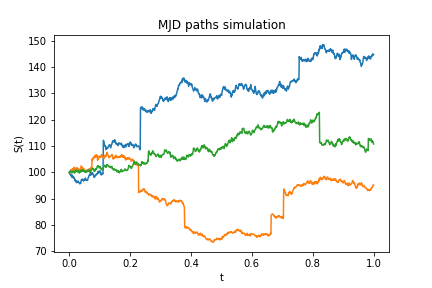
\includegraphics[scale = 0.6]{MS_Thesis_Template/figures/MJD_simulation.png}
    \caption{Simulation of MJD paths with $S_0=100, \mu=0.01,\sigma=0.1,\lambda=5,m=0$ and $\delta=0.1$.}
\label{mjd_paths}    
\end{figure}
Now when the time increment dt is small enough the distribution of (arithmetic) returns can be approximately computed using $e^x \approx 1 + x + \frac{x^{2}}{2}$, $(dB_t)^{2} = dt$ and ignoring terms of order higher than $dt$(in mean square sense). We illustrate it as follows:
\begin{align*}
R_{dt} = \frac{dS_t}{S_t} & = \frac{S_{t+dt}}{S_t} - 1 \\
& = \frac{e^{\left((\mu - \frac{1}{2} \sigma^{2})(t + dt) + \sigma B_{t+dt} +\sum_{i=1}^{N_{t+dt}} Y_i\right)}}{e^{\left((\mu - \frac{1}{2} \sigma^{2})t + \sigma B_{t} + \sum_{i= 1}^{N_{t}} Y_i\right)}} - 1 \\
& = e^{\left((\mu - \frac{1}{2} \sigma^{2}) dt + \sigma dB_t + \sum_{i=N_t + 1}^{N_{t+dt}} Y_i\right)} - 1\\
& \approx(\mu - \frac{1}{2} \sigma^{2}) dt + \sigma dB_t + \sum_{i=N_t + 1}^{N_{t+dt}} Y_i + \frac{1}{2} \Bigg(\Big[\Big(\mu - \frac{1}{2} \sigma^{2}\Big) dt\Big]^{2}\\
&~~ + 2 \Big(\mu - \frac{1}{2} \sigma^{2}\Big)\Big[\sigma dB_t + \sum_{i=N_t + 1}^{N_{t+dt}} Y_i\Big] dt  + \Big[\sigma dB_t + \sum_{i=N_t + 1}^{N_{t+dt}} Y_i\Big]^{2}\Bigg)\\
& \approx(\mu - \frac{1}{2} \sigma^{2}) dt + \sigma dB_t + \sum_{i=N_t + 1}^{N_{t+dt}} Y_i + \frac{1}{2}\Big[\sigma (dB_{t})^{2}\Big]\\
& =  \mu dt + \sigma dB_{t} + \sum_{i=N_t + 1}^{N_{t+dt}} Y_i.
\end{align*}
In the above expansion the terms with order higher than $dt$(in the mean square sense) has been droped off. Therefore the returns $R_{dt}$ approximately follows the distribution given by:  
\begin{equation}
\begin{aligned}
    R_{dt} &= \mu dt + \sigma dB_{t} + \sum_{i=N_t + 1}^{N_{t+dt}} Y_i\\
    & \stackrel{d}{=} \mu dt + \sigma dB_{t} + \sum_{i=1}^{dN_t} Y_i.\\
\end{aligned}
\label{approx_returns}    
\end{equation}
In above we have that $dN_t = N_{t+dt} - N_t $. Now since dt is small enough using definition of  poisson process (\ref{p_inc}) the term $dN_t$ either produces jump of size 1 with probability $\lambda dt$ or no jump with probability $1 - \lambda dt$. Therefore we have that 
\begin{equation}
 R_{dt} \stackrel{d}{=} \mu dt + \sigma \sqrt{dt}Z + BY.   
\end{equation}

where Z is standard normal random variable, $Y \stackrel{d}{=} \mathcal{N}(m,\delta^{2}) $  and $B$ is Bernoulli like random variable with $\mathbb{P}(B = 1) = \lambda dt$ and $\mathbb{P}(B = 0) = 1 - \lambda dt$.
Now on conditional on the event that $B=1$ and using the independence of $Z$ and $Y$ we have:
\begin{equation}
    R_{dt} \stackrel{d}{=} \mu dt + \sigma \sqrt{dt}.Z + Y \stackrel{d}{=} \mathcal{N}(\mu dt + m, \sigma^{2} dt + \delta^{2} ).   
\end{equation}
Similarly conditional on the event that $B=0$ we have:
\begin{equation}
    R_{dt} \stackrel{d}{=} \mu dt + \sigma \sqrt{dt}.Z  \stackrel{d}{=} \mathcal{N}(\mu dt, \sigma^{2} dt ).   
\end{equation}
Then the C.D.F. of $R_{dt}$  is given by:
\begin{align*}
    F_{R_{dt}}(x) = \mathbb{P}(R_{dt} \leq x) &= \mathbb{P}(R_{dt} \leq x | B =1) \mathbb{P}(B =1) + \mathbb{P}(R_{dt} \leq x | B = 0) \mathbb{P}(B =0)\\
    & = \lambda dt  \Phi\Bigg(\frac{x - (\mu dt + m)}{\sqrt{\sigma^{2} dt + \delta^{2}}}\Bigg) + (1 - \lambda dt) \Phi\Bigg(\frac{x-\mu dt}{\sigma \sqrt{dt}}\Bigg).
\end{align*}
This shows that the P.D.F. of returns under Merton jump diffusion model is given by,
\begin{equation}
    f_{R_{dt}}(x) =  \frac{\lambda dt}{\sqrt{\sigma^{2} dt + \delta^{2}}}  \phi\Bigg(\frac{x - (\mu dt + m)}{\sqrt{\sigma^{2} dt + \delta^{2}}}\Bigg) + \frac{(1 - \lambda dt)}{\sigma \sqrt{dt}} \phi\Bigg(\frac{x-\mu dt}{\sigma \sqrt{dt}}\Bigg).
\label{mjd_density}    
\end{equation}
where $\Phi$ and $\phi$ are the C.D.F. and P.D.F. respectively of standard normal random variable.
The below theorem gives the first four central moments of the returns.
\begin{theorem}[Theorem 5.17, \cite{hanson_2007}]
 Let $R_{dt}$ be the returns that satisfy \ref{approx_returns} and for convenience let $Y \stackrel{d}{=} Y_i$. Let $\mu_{j} = \E[Y]$ and $\sigma^{2}_j = \Var[Y]$ then the first four central moments are given by,\\
 \begin{equation}
     \begin{aligned}
       \E[R_{dt}] &= (\mu  + \mu_{j} \lambda) dt.\\
       \E[(R_{dt}- \E[R_{dt}])^{2}] &= (\sigma^{2} + (\sigma^{2}_j + \mu^{2}_{j}) \lambda) dt.\\
       \E[(R_{dt}- \E[R_{dt}])^{3}] &= \Big(\E[(Y- \mu_{j})^{3}] + (3 \sigma^{2}_j + \mu^{2}_{j}) \mu_{j}\Big)  \lambda dt.\\
       \E[(R_{dt}- \E[R_{dt}])^{4}] &= \Big(\E[(Y- \mu_{j})^{4}] + 4 \mu_j \E[(Y- \mu_{j})^{3}] + 6 \mu^{2}_{j} \sigma^{2}_j + \mu^{4}_j \Big) \lambda dt\\
       & ~~~~ + 3 (\sigma^{2} + (\sigma^{2}_j + \mu^{2}_{j})\lambda)^{2}(dt)^{2}.
     \end{aligned}
     \label{moments}
 \end{equation}
\end{theorem}
The above third and fourth central moments can be further simplified and are given by,
\begin{equation}
    \begin{aligned}
     \E[(R_{dt}- \E[R_{dt}])^{3}] &= (\E[Y^{3}])  \lambda dt.\\
     \E[(R_{dt}- \E[R_{dt}])^{4}] &= (\E[Y^{4}])\lambda dt + 3 (\sigma^{2} + (\sigma^{2}_j + \mu^{2}_{j})\lambda)^{2}(dt)^{2}.
    \end{aligned}
    \label{moments1}
\end{equation}
The mean, variance, skewness and excess kurtosis of the Merton jump diffusion modeled returns using \ref{moments} are given by,\\

\begin{equation}
    \begin{aligned}
    \E[R_{dt}] &= \mu dt + m \lambda dt. \\
    \Var[R_{dt}]& = \sigma^{2} dt + (\delta^{2} + m^2) \lambda dt.\\
    Skew[R_{dt}] &= \frac{\E[(R_{dt}- \E[R_{dt}])^{3}]}{(\Var[R_{dt}])^{\frac{3}{2}}}\\
    & = \frac{(3 \delta^{2} + m^{2}) m \lambda dt}{(\sigma^{2} dt + (\delta^{2} + m^2) \lambda dt)^{3/2}}.\\
    Excess~~Kurt[R_{dt}] &= \frac{\E[(R_{dt}- \E[R_{dt}])^{4}]}{(\Var[R_{dt}])^{2}} - 3\\
    & = \frac{(3 \delta^{4} + 6 m^{2} \delta^{2} + m^{4})\lambda dt}{(\sigma^{2} dt + (\delta^{2} + m^2) \lambda dt)^{2}}.
    \end{aligned}
\label{mjd_mean}    
\end{equation}
It is to be noted from the skewness in \ref{mjd_mean} that Merton jump diffusion model can capture the positive or negative skewness of the returns depending on the sign of $m$.We also note that the excess kurtosis of the model returns is non-zero provided $\lambda > 0 $. Thus the model also takes into account the heaviness of the tail of return distributions and a high value of $\lambda$ implies that the excess kurtosis will also be higher. Therefore the model tries to overcome some of the drawbacks that the Black Scholes model faces.  


\section{Kou Jump Diffusion Model}
S.G. Kou (\cite{kou_2002}) proposes the jump sizes of the compound poisson process in 4.4 to be given by a double exponential distribution.The jump size follows the distribution:
$$Y  \stackrel{d}{=} \left\{\begin{array}{lr}
        J^{+} & \text{with probability p }\\
        -J^{-} & \text{with probability q},
        \end{array}\right $$
where $J^{+} \stackrel{d}{=} exp(\eta_1) $ and $J^{-} \stackrel{d}{=} exp(\eta_2) $ where the former accounts for positive jumps with p probability and the latter accounts for negative jumps with q probability. The density of $Y$ is given by, 
\begin{equation}
f_Y(y)=p~\eta_1e^{-\eta_{1}y} \mathbb{I}_{\{y \geq 0\}}+q~\eta_2e^{ \eta_2 y } \mathbb{I}_{\{y < 0\}}, ~~~\eta_{1}>1,~\eta_{2}>0.
\label{y_density}
\end{equation}
Now using \ref{y_density} the following moments can be obtained. The condition $\eta_1 > 1$ is required for $E[V] < \infty$.
\begin{equation}
    \begin{aligned}
    \E[Y] & = \frac{p}{\eta_1} - \frac{q}{\eta_2}.\\
    \Var[Y] & = pq\Big(\frac{1}{\eta_1} + \frac{1}{\eta_2} \Big)^{2} + \Big(\frac{p}{\eta^{2}_1} + \frac{q}{\eta^{2}_2} \Big).\\
    \E[V] & = \E[e^{Y}]\\ 
    &= p \frac{\eta_1}{\eta_1 - 1} + q \frac{\eta_2}{\eta_2 + 1}.
    \end{aligned}
\end{equation}
Fig \ref{mjd_paths} shows simulation of paths of stock price process under Kou Jump Diffusion model.
\begin{figure}[H]
    \centering
    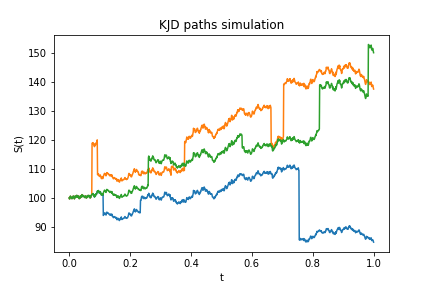
\includegraphics[scale = 0.6]{MS_Thesis_Template/figures/KJD_simulation.png}
    \caption{Simulation of KJD paths with $S_0 =100, \mu=0.01,\sigma=0.1,\lambda=5,p=0.5,\eta_1=10$ and $\eta_2=10$.}
\label{kjd_paths}    
\end{figure}
Now using the distributional approximation $R_{dt} \stackrel{d}{=} \mu dt + \sigma \sqrt{dt}Z + BY$ we will derive the density of the returns. Similar to the previous case when conditional on the event $B = 0$, the returns are distributed as $R_{dt} \stackrel{d}{=} \mu dt + \sigma \sqrt{dt}Z$ which implies that the density of returns in this case is given by $\frac{1 - \lambda dt}{\sigma \sqrt{dt}} \phi\left(\frac{x- \mu dt}{\sigma \sqrt{dt}}\right)$. Now conditional on the event $B=1$, we have that the returns are distributed as $R_{dt} \stackrel{d}{=} \mu dt + \sigma \sqrt{dt}Z + Y \stackrel{d}{=} N + Y $ which is the sum of independent normal random variable (N) and a double exponentially distributed random variable(Y) respectively where $N \stackrel{d}{=} \mathcal{N}(\mu dt, \sigma^{2} dt )$. Then the density of $N+Y$ is given by the convolution of the densities of $N$ and $Y$ respectively we illustrate it as follows:\\
\begin{aligned}
f_{N+Y}(x) &= (f_{N}*f_{Y})(x)\\ & = \int \limits _{-\infty }^{\infty } f_{N}(x-y)~f_{Y}(y)~dy\\
& = \int \limits _{-\infty }^{\infty } \frac{1}{\sqrt{2 \pi \sigma^{2} dt}} e^{-\frac{(x-y-\mu dt)^{2}}{2 \sigma^{2} dt}} \Big[p~\eta_1e^{-\eta_{1}y} \mathbb{I}_{\{y \geq 0\}}+q~\eta_2e^{ \eta_2 y } \mathbb{I}_{\{y < 0\}}\Big]~dy\\
& = p\eta_1\int \limits _{0 }^{\infty }\frac{1}{\sqrt{2 \pi \sigma^{2} dt}}e^{\frac{-y^{2} + 2y(x-\mu dt) - (x-\mu dt)^{2} - 2\eta_1 y \sigma^{2} dt}{2 \sigma^{2} dt}} ~dy\\
&~~~~~~~~~+ q\eta_2\int \limits _{-\infty }^{0}\frac{1}{\sqrt{2 \pi \sigma^{2} dt}}e^{\frac{-y^{2} + 2y(x-\mu dt) - (x-\mu dt)^{2} + 2\eta_2 y \sigma^{2} dt}{2 \sigma^{2} dt}} ~dy \\
& = p\eta_1 e^{-\frac{(x - \mu dt)^{2}}{2 \sigma^{2} dt}}\int \limits _{0 }^{\infty }\frac{1}{\sqrt{2 \pi \sigma^{2} dt}}e^{\frac{-y^{2} + 2y(x-\mu dt - \eta_1 \sigma^{2} dt)}{2 \sigma^{2} dt}} ~dy\\
&~~~~~~~~~+ q\eta_2 e^{-\frac{(x - \mu dt)^{2}}{2 \sigma^{2} dt}}\int \limits _{-\infty }^{0}\frac{1}{\sqrt{2 \pi \sigma^{2} dt}}e^{\frac{-y^{2} + 2y(x-\mu dt + \eta_2 \sigma^{2} dt)}{2 \sigma^{2} dt}} ~dy \\
& = p\eta_1 e^{-\frac{(x - \mu dt)^{2}}{2 \sigma^{2} dt}} e^{\frac{(x-\mu dt - \eta_1 \sigma^{2} dt)^{2}}{2 \sigma^{2} dt}}\int \limits _{0 }^{\infty }\frac{1}{\sqrt{2 \pi \sigma^{2} dt}}e^{\frac{-(y-(x-\mu dt - \eta_1 \sigma^{2} dt))^{2}}{2 \sigma^{2} dt}} ~dy\\
&~~~~~~~~~+ q\eta_2 e^{-\frac{(x - \mu dt)^{2}}{2 \sigma^{2} dt}} e^{\frac{(x-\mu dt + \eta_2 \sigma^{2} dt)^{2}}{2 \sigma^{2} dt}}\int \limits _{-\infty }^{0}\frac{1}{\sqrt{2 \pi \sigma^{2} dt}}e^{\frac{-(y-(x-\mu dt + \eta_2 \sigma^{2} dt))^{2}}{2 \sigma^{2} dt}} ~dy \\
& = p \eta_{1} e^{\frac{\sigma^{2} \eta_1^{2} dt}{2}} e^{-(x-\mu dt)\eta_1} \Phi\left(\frac{x - \mu dt - \sigma^{2} \eta_1 dt}{\sigma \sqrt{dt}}\right)\\ 
&~~~~~~~~~ + q \eta_{2} e^{\frac{\sigma^{2} \eta_2^{2} dt}{2}} e^{(x-\mu dt)\eta_2} \Phi\left(\frac{-(x - \mu dt + \sigma^{2} \eta_2 dt)}{\sigma \sqrt{dt}}\right).


\end{aligned}

 Therefore the density of returns for Kou Jump Diffusion model is given by:
\begin{equation}
\begin{aligned}
f_{R_{dt}}(x) = &\frac{1 - \lambda dt}{\sigma \sqrt{dt}} \phi\left(\frac{x- \mu dt}{\sigma \sqrt{dt}}\right) + \lambda dt \Bigg\{p \eta_{1} e^{\frac{\sigma^{2} \eta_1^{2} dt}{2}} e^{-(x-\mu dt)\eta_1} \Phi\left(\frac{x - \mu dt - \sigma^{2} \eta_1 dt}{\sigma \sqrt{dt}}\right)\\ 
& + q \eta_{2} e^{\frac{\sigma^{2} \eta_2^{2} dt}{2}} e^{(x-\mu dt)\eta_2} \Phi\left(\frac{-(x - \mu dt + \sigma^{2} \eta_2 dt)}{\sigma \sqrt{dt}}\right) \Bigg\}.
\end{aligned}
\label{kou_density}
\end{equation}
where $\phi$ and $\Phi$ are the P.D.F. and C.D.F. of standard normal random variable respectively.

The mean, variance, skewness and excess kurtosis of the Kou jump diffusion modeled returns using \ref{moments}  and \ref{moments1} are given by,\\
\begin{equation}
    \begin{aligned}
    \E[R_{dt}] &= \mu dt +  \Big(\frac{p}{\eta_1} - \frac{q}{\eta_2}\Big)\lambda dt. \\
    \Var[R_{dt}]& = \sigma^{2} dt + \Big\{pq\Big(\frac{1}{\eta_1} + \frac{1}{\eta_2} \Big)^{2} + \Big(\frac{p}{\eta^{2}_1} + \frac{q}{\eta^{2}_2} \Big)\Big\} \lambda dt \\
    & + \Big(\frac{p}{\eta_1} - \frac{q}{\eta_2} \Big)^{2} \lambda dt.\\
    Skew[R_{dt}] &= \frac{\E[(R_{dt}- \E[R_{dt}])^{3}]}{(\Var[R_{dt}])^{\frac{3}{2}}}\\
    & = \frac{6 \Big(\frac{p}{\eta^{3}_1} - \frac{q}{\eta^{3}_2 }\Big)  \lambda dt}{(\Var[R_{dt}])^{\frac{3}{2}}}.\\
    Excess~~Kurt[R_{dt}] &= \frac{\E[(R_{dt}- \E[R_{dt}])^{4}]}{(\Var[R_{dt}])^{2}} - 3\\
    & = \frac{24 \Big(\frac{p}{\eta^{4}_1}\Big + \frac{q}{\eta^{4}_2} \Big) \lambda dt}{(\Var[R_{dt}])^{2}}.
    
    \end{aligned}
\label{kjd_mean}    
\end{equation}

From \ref{kjd_mean} it can be noted that the Kou Jump diffusion model also tries to capture the non-zero skewness of the returns distribution and the non-zero excess kurtosis (provided $\lambda > 0$) suggests that the model also tries to capture the heaviness of the tails of the returns distribution.
\section{Option pricing under Jump Diffusion Models and parameter estimation}
We know from section \ref{jdsde} that the stock price process under jump diffusion model is given by,\\
\begin{equation}
S_t=S_0‎\exp‎\Big\{(\mu- ‎\frac{1}{2}‎\sigma‎^2‎)t+‎\sigma ‎B_t‎\Big\} ‎\prod‎_{i=1}^{N_t}V_i.
\label{st_price}
\end{equation}
We first compute $\E[\prod‎_{i=1}^{N(t)}V_i]$ as follows:

\begin{aligned}
\E[\prod‎_{i=1}^{N(t)}V_i]  = \E[\E[\prod‎_{i=1}^{N(t)}V_i|N(t)]]
& = \sum_{n=0}^{\infty} \E[\prod‎_{i=1}^{N(t)}V_i|N(t)=n].\mathbb{P}(N(t)=n)\\
& = \sum_{n=0}^{\infty} \E[\prod‎_{i=1}^{n}V_i]. \frac{e^{-\lambda t}(\lambda t)^{n}}{n!}\\
& = e^{-\lambda t} \sum_{n=0}^{\infty} (E[V_i])^{n}. \frac{(\lambda t)^{n}}{n!}\\
& = e^{-\lambda t (1 - \E[V_i])}.
\end{aligned}

Now for pricing the options we want $\{e^{-rt}S_t , t >0\}$ to be a martingale. We will find the condition under which the discounted stock price process in \ref{st_price} becomes a martingale. Suppose $\{e^{-rt}S_t , t >0\}$ is a martingale then it must have constant expectation which implies that\\
$~~~~~~~~~~~~~~~~~~~~~~~~~~~\E[e^{-rt}S_t] = S_0 \iff &e^{-rt} S_0 e^{\mu t} e^{-\lambda t (1 - \E[V_i])} = S_0$\\
$~~~~~~~~~~~~~~~~~~~~
~~~~~~~~~~~~~~~~~~~~~~~~~~\iff e^{(\mu - r - \lambda (1 - \E[V_i]))t} = 1\\$
$~~~~~~~~~~~~~~~~~~~~
~~~~~~~~~~~~~~~~~~~~~~~~~~\iff \mu = r - \lambda(\E[V_i - 1])$. \\
We denote $\E[V_i - 1]$ by $k$. Therefore the risk neutral stock price process is given by,
\begin{equation}
S_t=S_0‎\exp‎\Big\{(r - \lambda k- ‎\frac{1}{2}‎\sigma‎^2‎)t+‎\sigma ‎B_t‎\Big\} ‎\prod‎_{i=1}^{N_t}V_i. \label{risk_neutral}   
\end{equation}
Let $K$ be the strike price and $T$ be the maturity time of call option. Then the call option price at t=0 under the jump diffusion models is given by,
\begin{equation}
    C(0,S_0) = \E[e^{-rT} (S_T - K)^{+}],
\label{monte_carlo}    
\end{equation}
 where $S_T$ is given by the risk neutral stock price process \ref{risk_neutral}.\\
Now for parameter estimation we have used the M.L.E. method. Let $\{x_1,x_2,...,x_n\}$ be the empirical (arithmetic) returns then the parameters of the models will be estimated by maximising the likelihood function,
\begin{equation}
    L =  \prod\limits_{i=1}^n f_{R_{dt}}(x_i).
\end{equation}
For Merton jump diffusion model the density in \ref{mjd_density} will be used for the likelihood and similarly for Kou Jump diffusion model the density in \ref{kou_density}  will be used for the likelihood. Further in this case the initial estimates of the parameters are required for optimisation purpose. To deal with this we have used the methodology and approach discussed in \cite{tang_2018}. 


 
\label{jd_mle}

\section{Application of the Black Scholes and the Jump Diffusion models for Infosys stock}
In this section we will cover the application of the Black scholes, Merton jump diffusion and Kou jump diffusion models for Infosys stock. We will be using around 8 years
of historical data (01/01/2014 - 21/04/2022 ) of closing prices of Infosys stock \footnote{Historical data of closing price of Infosys has been obtained from https://finance.yahoo.com}. Fig \ref{infy_data} shows daily closing price of the Infosys stock from 2014-01-01.

\begin{figure}[H]
    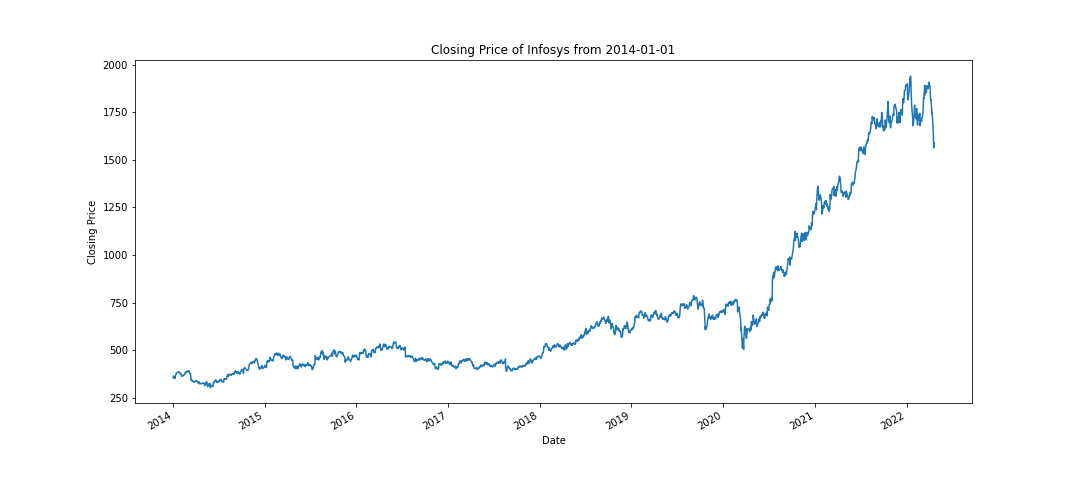
\includegraphics[scale=0.45]{MS_Thesis_Template/figures/INFY_closing prices.png}
    \caption{Daily closing price of Infosys stock.}
\label{infy_data}    
\end{figure}   


\subsection{Parameter estimation and comparative study of the models}
In this section we will estimate the parameters of BS, MJD and KJD models respectively.After estimation process we will then do a comparative study to conclude which model fits better to the Infosys stock. Fig \ref{rel_returns} shows the daily (arithmetic) returns of Infosys stock from 2014-01-01.
\begin{figure}[H]
    \centering
    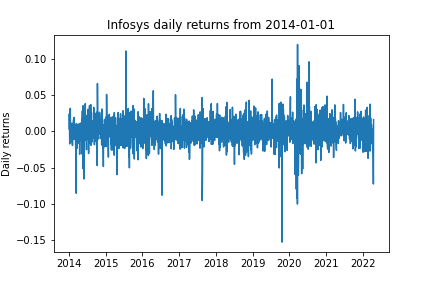
\includegraphics[scale = 0.6]{MS_Thesis_Template/figures/INFY_daily_returns.png}
    \caption{Daily returns of Infosys stock.}
\label{infy_returns}    
\end{figure}
Table \ref{infy_stats} shows some statistics of the daily returns of Infosys stock. Negative value of skewness suggests that the distribution of returns is skewed to left side rather than being symmetric. High kurtosis of returns suggests that the distribution of returns have heavier tails which means that the tail of the returns distribution dies
out slowly.

\begin{table}[H]
\centering
\begin{tabularx}{0.7\textwidth}
{ 
  | >{\raggedright\arraybackslash}X 
  | >{\raggedright\arraybackslash}X 
  | >{\raggedright\arraybackslash}X
  | >{\raggedright\arraybackslash}X
  |}
  \hline
   Mean & Variance & Skewness & Kurtosis \\
  \hline
    0.000881    & 0.000292    & -0.299524  & 11.922975  \\
  \hline
\end{tabularx}
\caption{Some statistics of daily returns of Infosys stock.}
\label{infy_stats}
\end{table}
We now use the M.L.E. method discussed in section \ref{bs_mle} to estimate the BS model parameters. Table \ref{bs_para} shows the estimated $\mu$ and $\sigma$. 

\begin{table}[H]
\centering
\begin{tabularx}{0.5\textwidth}
{ 
  | >{\raggedright\arraybackslash}X 
  | >{\raggedright\arraybackslash}X 
  |}
  \hline
   \mu & \sigma \\
   \hline
   0.258676       & 0.271156  \\
   
   \hline
\end{tabularx}
\caption{BS estimated parameters.}
\label{bs_para}
\end{table}
Table \ref{mjd_para} and \ref{kjd_para} shows the estimated parameters of the MJD and the KJD models respectively using the M.L.E. method discussed in section \ref{jd_mle}
\begin{table}[H]
\centering
\begin{tabularx}{1.1\textwidth}
{ 
  | >{\raggedright\arraybackslash}X 
  | >{\raggedright\arraybackslash}X 
  | >{\raggedright\arraybackslash}X 
  | >{\raggedright\arraybackslash}X
  | >{\raggedright\arraybackslash}X 
  | >{\raggedright\arraybackslash}X 
  |}
  \hline
   \mu & \sigma & \lambda & m         & \delta  \\
   \hline
   0.253644       & 0.205033    & 18.628368    &-0.001703              & 0.041080    \\
   
   \hline
\end{tabularx}
\caption{MJD estimated parameters through M.L.E.}
\label{mjd_para}
\end{table}

\begin{table}[H]
\centering
\begin{tabularx}{1.1\textwidth}
{ 
  | >{\raggedright\arraybackslash}X 
  | >{\raggedright\arraybackslash}X 
  | >{\raggedright\arraybackslash}X 
  | >{\raggedright\arraybackslash}X
  | >{\raggedright\arraybackslash}X 
  | >{\raggedright\arraybackslash}X 
  |}
  \hline
   \mu & \sigma & \lambda & p         & \eta_1           & \eta_2         \\
   \hline
   0.106614       & 0.190477    & 49.741324    & 0.630307             & 59.434328             & 44.687403 \\
   
   \hline
\end{tabularx}
\caption{KJD estimated parameters through M.L.E.}
\label{kjd_para}
\end{table}
Then using the estimated parameters we then generated simulations of returns from each of the models.Fig \ref{returns_sim} shows the plots of the simulated returns from each model and its comparison with the empirical returns. 

\begin{figure}[H]
    \centering
    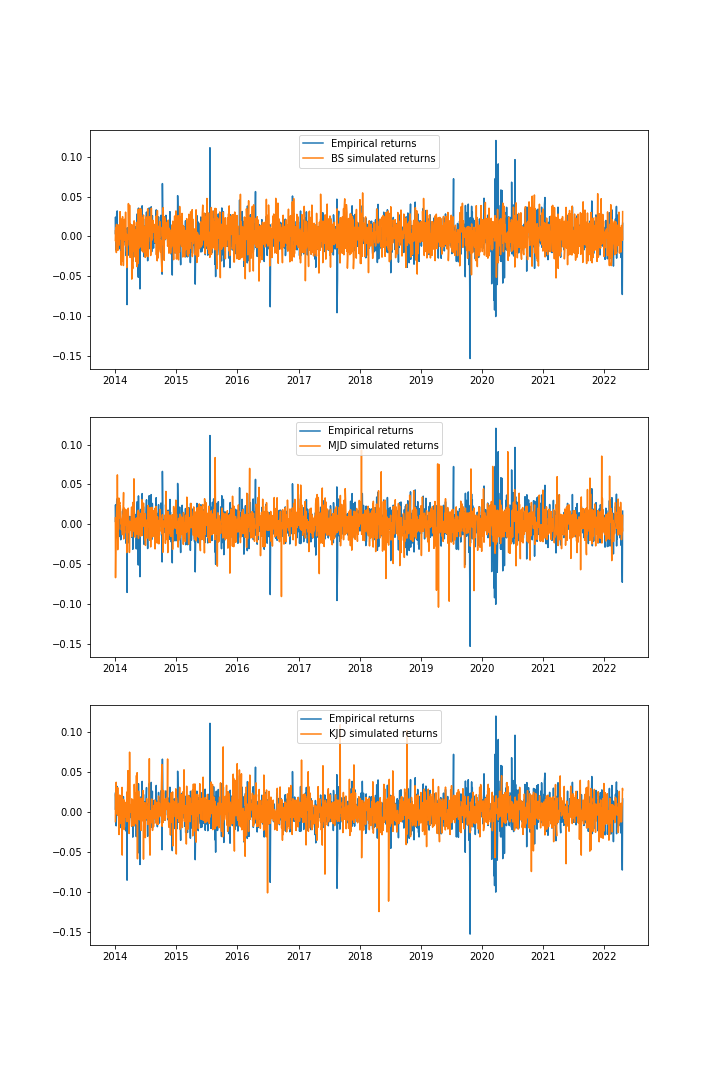
\includegraphics[width = 16cm,height=15.5cm]{MS_Thesis_Template/figures/simulated_returns.png}
    \caption{Comparison of the empirical returns with the simulated returns of the BS,  MJD and KJD models
    respectively.}
\label{returns_sim}    
\end{figure}
From fig \ref{returns_sim} we can observe that the BS model fails to capture the occasional spikes(jump points) that are present in the empirical returns.The MJD and KJD models on the other hand show some occasional spikes in the plots indicating that they can model the occasional jumps of Infosys stock returns. We then covered the distributional comparison of the empirical returns with that of the returns modeled from each of the three models.Fig \ref{kde} shows the Kernel Density Estimate plot of the empirical returns and the simulated returns of fig \ref{returns_sim} from each models.    
\begin{figure}[H]

    \hspace{-3cm}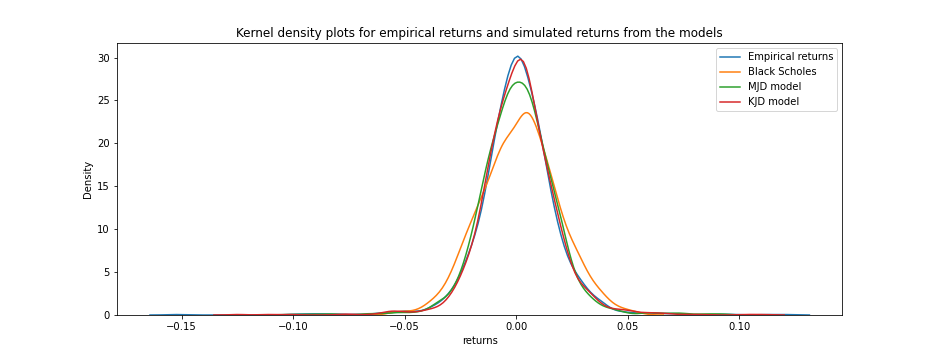
\includegraphics[scale = 0.7]{MS_Thesis_Template/figures/KDE_plot_INFY.png}
    \caption{Comparison of the kernel density estimate plots of empirical returns with the BS, MJD and KJD models simulated returns respectively.}
\label{kde}    
\end{figure}
The K.D.E. plot suggests that the density of MJD and the KJD simulated returns fits better to that of the empirical returns as compared to the BS simulated returns density. It can be observed that the KJD model better captures the peak of the empirical returns distribution and also the tails of the KJD distribution is heavier than the other models.
We then computed some statistics implied by each of the three models using \ref{bs_mean},\ref{mjd_mean} and \ref{kjd_mean}.
Table \ref{jd_stats} shows the computed statistics and its comparison with that of empirical returns.

\begin{table}[H]
\centering
\begin{tabularx}{1.1\textwidth}
{ 
  | >{\raggedright\arraybackslash}X 
  | >{\raggedright\arraybackslash}X 
  | >{\raggedright\arraybackslash}X 
  | >{\raggedright\arraybackslash}X
  | >{\raggedright\arraybackslash}X 
  |}
  \hline
   & Mean & Variance & Skewness & Kurtosis  \\
   \hline
   Empirical Returns & 0.000881    & 0.000292    & -0.299524  & 11.922975    \\
    \hline
   BS Model & 0.000881    & 0.000292    &0  & 3    \\
    \hline
   MJD Model & 0.000881    & 0.000292    &-0.127939  & 10.443763    \\
    \hline
   KJD Model & 0.000883    & 0.000287    &-0.277089  & 11.208304    \\
    \hline
   
   \hline
   
\end{tabularx}
\caption{Comparison of some statistics of the BS, MJD and KJD modelled returns respectively with the empirical returns. }
\label{jd_stats}
\end{table}

It can be noted through the kurtosis values that the MJD and the KJD captures the heaviness of the tail of the distribution of returns and the heaviness of tails is more pronounced in the case of KJD model which the BS model fails to capture. Similarly both the MJD and KJD model respectively captures the negative skewness of the Infosys returns and the value of skewness of KJD model is more close to that of the Infosys returns as compared to the MJD model. Therefore comparatively we can conclude that the KJD model is a better fit for the Infosys stock data.  

\subsection{Pricing Infosys Call options under the BS and the Jump diffusion models\footnote{Call options data of Infosys has been obtained from https://www.nseindia.com/option-chain}}
In this section we will be pricing some Infosys call options dated 21/04/2022 using the estimated BS, MJD and KJD model of the previous section. For BS model the closed form pricing formula \ref{bs_call_price} will be used. The call price under MJD and KJD model using \ref{monte_carlo} and the central limit theorem can be approximated by,
\begin{equation}
    Price = e^{-rT} \Big(\frac{\sum_{i=1}^N (S_T - K)^{+}}{N}\Big).
\label{price}    
\end{equation}
where $S_T$ follows the risk neutral equity process as mentioned in \ref{risk_neutral}. We simulated N=100000 values of $S_T$ and computed the call option prices for MJD and KJD model using \ref{price}. The initial price $S_0$ was 1615.70 rupees on 21-04-2022 with expiry on 26-05-2022.We have taken r = 0.045 which is the current 1-Year Government Bond Yield.
Table \ref{jd_price} shows the computed option prices of the three models for varying strike prices of Infosys call options. We can note that all the three models performs fine in terms of pricing and the prices are close to the MID PRICES. 

\begin{table}[H]
\centering
\begin{tabularx}{1\textwidth}
{ 
  | >{\raggedright\arraybackslash}X 
  | >{\raggedright\arraybackslash}X 
  | >{\raggedright\arraybackslash}X 
  | >{\raggedright\arraybackslash}X
  | >{\raggedright\arraybackslash}X 
  | >{\raggedright\arraybackslash}X 
  | >{\raggedright\arraybackslash}X
  |}
   \hline
   STRIKE PRICE & BID PRICE & ASK PRICE & MID PRICE & BS PRICE  & MJD PRICE & KJD PRICE \\
   \hline
   1500.0       & 132.7     & 135.85    & 134.275   & 134.40275 & 134.8983  & 134.27881 \\
   \hline
   1520.0       & 111.55    & 121.3     & 116.425   & 118.62497 & 119.20429 & 118.17841 \\
   \hline
   1540.0       & 101.05    & 103.5     & 102.275   & 103.79511 & 102.97129 & 102.97846 \\
   \hline
   1560.0       & 87.7      & 88.75     & 88.225    & 90.0016   & 88.9934   & 90.07431  \\
   \hline
   1580.0       & 73.9      & 75.35     & 74.625    & 77.31336  & 76.58405  & 76.77823  \\
   \hline
   1600.0       & 61.8      & 62.85     & 62.325    & 65.77603  & 65.53064  & 64.64055  \\
   \hline
   1620.0       & 52.1      & 52.5      & 52.3      & 55.40992  & 54.75655  & 54.19889  \\
   \hline
   1640.0       & 42.55     & 43.0      & 42.775    & 46.20955  & 45.66211  & 45.45656  \\
   \hline
   1660.0       & 34.65     & 35.4      & 35.025    & 38.14495  & 37.53703  & 37.3841   \\
   \hline
   1680.0       & 28.0      & 28.8      & 28.4      & 31.16438  & 30.70015  & 30.18425  \\
   \hline
   1700.0       & 22.75     & 22.9      & 22.825    & 25.19812  & 24.85551  & 24.33266  \\
   \hline
   1720.0       & 18.25     & 18.75     & 18.5      & 20.16294  & 19.81938  & 19.51125  \\
   \hline
   1740.0       & 14.55     & 14.9      & 14.725    & 15.96678  & 15.77687  & 15.12316  \\
   \hline
   1760.0       & 12.0      & 12.35     & 12.175    & 12.51337  & 12.44429  & 12.09165 \\
   \hline
\end{tabularx}
\caption{Computed Option prices of Infosys call options under BS, MJD and KJD models respectively.}
\label{jd_price}
\end{table}

\textbf{Note:} Since we are relying on simulations for pricing in case of MJD and KJD model using \ref{price}. The prices under the next scenario of simulations might change but not by an insignificant amount.




\chapter{Volatility}

\section{The Implied Volatility}
Let $C(S_{0},K,T,r,\sigma)$ be the Black Scholes price of a call option with $S_0,K$ and $T$ as the initial price of stock, strike price and maturity time of the option respectively. Let $M$ denote the market price of the call option. Then the implied volatility denoted is the value of $\sigma$ that makes the two prices equal i.e.,
\begin{equation}
    C(S_{0},K,T,r,\sigma) = M.
\end{equation}
Now from the Black Scholes formula it is not possible to express $\sigma$ in terms of the other parameters and the Black Scholes price in closed form. We can compute $\frac{\partial C}{\partial \sigma}$ and is given by,
\begin{equation}
    \frac{\partial C}{\partial \sigma} = S_0 \sqrt{T} \phi(d_1),
\end{equation}
where $\phi$ is standard normal density and $d_1$ is given by \ref{d_1}.  This implies that $\frac{\partial C}{\partial \sigma} > 0$, which means that the Black Scholes price is a monotonic increasing function of $\sigma$. Therefore to compute the implied volatility of a call option we can use Newton-Raphson method of root finding for the function $f(\sigma) = C(S_{0},K,T,r,\sigma) - M$. The Newton-Raphson method for a function $f(x)$ to estimate its root first requires an interval $(a,b)$ in which its root lies. Then with an initial guess of root $x_0 = \alpha$ where $\alpha \in (a,b)$. The root is estimated by the following iteration:
\begin{equation}
    x_{n+1} = x_{n} - \frac{f(x_n)}{f^{'}(x_n)} , ~~~~f^{'}(x_n) \neq 0. 
\end{equation}
Fig \ref{tata} shows the computed implied volatility(using Newton Raphson method) plot of TATA MOTORS call options\footnote{Call options data used in this section has been obtained from https://www.nseindia.com/option-chain and as per the convention of NSE option chain site r = 10\% is used for computing the implied volatility.} dated 28-01-22 with $S_0 = 497.30$ and maturity $T=27$ days. For comparison NSE Option Chain site implied volatility values is also plotted. We can observe from the plot that Newton-Raphson method works well for computing implied volatility.    




\begin{figure}[H]
    \centering
    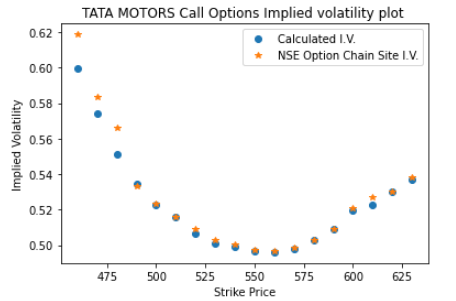
\includegraphics[scale = 0.6]{MS_Thesis_Template/figures/TATA_IV_plot.png}
    \caption{TATA MOTORS stock call options implied volatility plot.}
\label{tata}    
\end{figure}
Fig \ref{nifty} shows the implied volatility plot of NIFTY50 stock index call options dated 29-11-21 with $S_0=17053.9$ and $T=3,10,17,31$ days. The volatility surface plot which is a plot between the implied volatility, strike price and maturities is also plotted.\footnote{The computed implied volatility used for plotting for both TATA MOTORS and NIFTY50 stock is shown in Appendix \ref{app:appendix2}}


\begin{figure}[H]
    \centering
    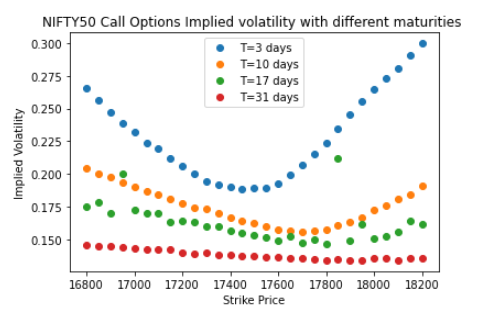
\includegraphics[scale = 0.6]{MS_Thesis_Template/figures/NIFTY50_IV_plot.png}
    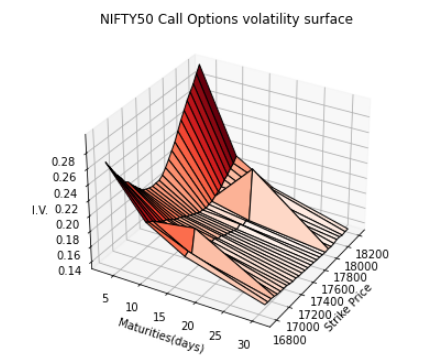
\includegraphics[scale = 0.6]{MS_Thesis_Template/figures/Nifty_vol_surface.png}
    \caption{NIFTY50 stock index call options implied volatility and volatility surface plot.}
\label{nifty}    
\end{figure}

Now if the Black Scholes assumption that $\sigma$ is constant was true then we would have obtained a flat line in the implied volatility plot but in general it is usually observed that the implied volatility plot is in the shape of a smile or it is skewed to one of the side as observed in Fig \ref{tata} and \ref{nifty}. This suggests that $\sigma$
atleast as a function of $K$ and $T$ is not constant. One of reason for obtaining smile in the implied volatility plot is that the demands of in the money or out of the money options are more as compared to at the money options which led to more pricing of these options as compared to at the money options and as a result of that the implied volatility is more for these options. For a more detailed discussion on implied volatility the reader is encouraged to refer to \cite{hull_2018} and \cite{papanicolaou_2019}.\\
In the next section we discuss the GARCH models which are used to model time varying volatilty. Theory for the next section is covered from \cite{tsay_2016}.
\section{GARCH(1,1) Model}
GARCH stands for Generalised Autoregressive Conditional  Heteroskedasticity. In layman terms heteroskedasticity means volatility. Under GARCH the present volatility of the series depends on its past. GARCH model requires the assumption of stationarity (in the weak sense) of the series. 
In a GARCH(1,1) model\footnote{In general a GARCH$(p,q)$ model involves $p$ lag terms and $q$ lag terms of $r_t$ and $\sigma_t$ respectively in 5.4. We have restricted our study to GARCH$(1,1)$ model only for this project.} the log-return series $r_t$ follows:\\
\begin{equation}
 r_t = \sigma_t \epsilon_t ,~~~~~~ \sigma^{2}_t = \omega + a r^{2}_{t-1} + b \sigma^{2}_{t-1}. 
\label{garch_sigma} 
\end{equation}
where $\{\epsilon_t\}_{t >0}$ is a sequence of i.i.d. random variables (also known as innovations or noise) with mean 0 and variance 1 and $\omega = \gamma V_L$ where $V_L$ is the long run variance.Usually we have that $\epsilon_t \stackrel{d}{=} \mathcal{N}(0,1)$.We have the following conditions on the parameters $\omega > 0,a \geq 0,b \geq 0 $,$(a + b) < 1$ and $\gamma + a + b =1$.The terms  $\sigma^{2}_t$ measures the conditional variance of the series $r_t$ we will show this. Let $\mathcal{F}_t$ denote the information about $\sigma_t$ till time $t$ then the conditional mean\footnote{The GARCH model also involves modeling the conditional mean of $r_t$. In this project we have only considered the case when the conditional mean of $r_t$ is zero.} and conditional variance of $r_t$ is given by,\\
$$E[r_t|\mathcal{F}_{t-1}] = \sigma_t E[\epsilon_t|\mathcal{F}_{t-1}] = \sigma_t E[\epsilon_t] = 0.$$
\begin{align*}
Var[r_t|\mathcal{F}_{t-1}] &= E[(r_t - E[r_t|\mathcal{F}_{t-1}] )^{2}|\mathcal{F}_{t-1}]\\
& = E[r_t^{2}|\mathcal{F}_{t-1}]\\
& = \sigma_t^{2} E[\epsilon_t^{2}|\mathcal{F}_{t-1}]\\
& = \sigma_t^{2} E[\epsilon_t^{2}]\\
& = \sigma_t^{2}.
\end{align*}
Now using law of total expectation and variance we can show the following,
\begin{align*}
E[r_t] & = E[E[r_t|\mathcal{F}_{t-1}]]\\
& = E[\sigma_t E[\epsilon_t|\mathcal{F}_{t-1}]]\\
& = 0.\\
Var[r_t] & = E[Var[r_t|\mathcal{F}_{t-1}]] + Var[E[r_t|\mathcal{F}_{t-1}]]\\
& = E[\sigma_t^{2}] + 0\\
& = E[\sigma_t^{2}].
\end{align*}
From above it follows that $Var[r_t] = E[r_t^{2}] = E[\sigma_t^{2}]$. Now using this and the assumption of stationarity of the series $r_t$ we can compute the unconditional variance as follows:\\
\begin{align*}
    Var[r_t] & = E[\sigma_t^{2}]\\
    & = E[\omega + a r^{2}_{t-1} + b \sigma^{2}_{t-1}]\\
    & = \omega + a E[r^{2}_{t-1}] + b E[r^{2}_{t-1}]\\
    & = \omega + a E[r^{2}_{t}] + b E[r^{2}_{t}]\\
    & = \omega + a Var[r_{t}] + b Var[r_{t}].\\
\end{aligned*}\\
This gives,
\begin{equation}
    Var[r_t] = \frac{\omega}{1 -a -b}.
\end{equation}
The restriction $a + b < 1$ is required for  $Var[r_t]$ in 5.5 to be well defined. It can be observed that the unconditional variance $Var[r_t]$ is same as the long run variance $V_L$. The GARCH(1,1) model is a mean reverting model. The variance tends to get pulled towards the long run variance $V_L$ with time and the speed of the reversion is governed by the parameter $\gamma$. For more detail to the mean reversion property of GARCH(1,1) model the reader is encouraged to refer to \cite{hull_2018}. \\
GARCH(1,1) model also captures the phenomena of volatility clustering in which large changes of volatility tends to be followed by large  changes of volatility and similarly for the small changes of volatility .This can be observed from 5.4 that large value of $\sigma^{2}_{t-1}$ or $r^{2}_{t-1}$ will result in large value of $\sigma_{t}$ in next period and similar reason for small values as well.\\
Now for the noise terms $\epsilon_t$ we have that,
$$E[\epsilon^{4}_t] = K_{\epsilon} + 3,$$
where $K_{\epsilon}$ is the excess kurtosis of the noise terms. Then,\\
$$E[r^{4}_t] = E[\sigma^{4}_t] E[\epsilon^{4}_t] = (K_{\epsilon} + 3) E[\sigma^{4}_t].$$
Using 5.4 it can be shown that,\\
$$E[\sigma^{4}_t] = \frac{\omega^{2}(1 + a + b)}{(1-a-b)(1 - (a + b)^{2} - a^{2}(K_{\epsilon} + 2))}.$$ 
\textbf{Note:} We require $a+b < 1$ and $(1 - (a + b)^{2} - a^{2}(K_{\epsilon} + 2)) > 0 $ for the existence of $E[\sigma^{4}_t]$. The Kurtosis of the GARCH(1,1) modelled returns denoted by $K_r$ is found to be,\\
$$K_r = \frac{E[r^{4}_t]}{(Var[r_t])^2} = \frac{(K_{\epsilon} + 3)(1 - (a + b)^{2})}{(1 - 2 a^{2} - (a + b)^{2} -K_{\epsilon}a^{2})}.$$
Since $K_{\epsilon} \geq 0$ then we have that,\\
$$K_r = \frac{(K_{\epsilon} + 3)(1 - (a + b)^{2})}{(1 - (a + b)^{2} - 2 a^{2} -K_{\epsilon}a^{2})} > \frac{(K_{\epsilon} + 3)(1 - (a + b)^{2})}{(1 - (a + b)^{2})} > (K_{\epsilon} + 3) \geq 3. $$
This shows that the distribution of  $r_t$ under GARCH(1,1) model have heavier tails than that implied by normal distribution. Now if $\epsilon_t \stackrel{d}{=} \mathcal{N}(0,1) $ then $ K_{\epsilon} = 0$ and the kurtosis of $r_t$ denoted by $K^{g}_r$ is given by,\\
\begin{equation}
 K^{g}_r = \frac{ 3 (1 - (a + b)^{2})}{(1 - 2 a^{2} - (a + b)^{2})}. 
\label{gauss_kurt} 
\end{equation}
In order to account for more heavier tails of distribution of $r_t$, Student's t distribution with $\nu$ degrees of freedom can be used for the distribution of noise terms. In this case $K_{\epsilon} = \frac{6}{\nu - 4}$ and the kurtosis of $r_t$ denoted by $K^{t}_r$ is given by,\\
\begin{equation}
  K^{t}_r = \frac{(\frac{6}{\nu - 4} +3) (1 - (a + b)^{2})}{(1 - 2 a^{2} - (a + b)^{2} - \frac{6}{\nu - 4} a^{2})}.
\label{t_kurt} 
\end{equation}


\subsection{Parameter estimation}
The parameters of the GARCH(1,1) model can be estimated by M.L.E. method. Let $\{x_1,x_2,...,x_n\}$ be the empirical log-returns. The methodology is to maximise the following likelihood function,\\
\begin{equation}
    L =  \prod\limits_{i=1}^n f_{r_{t}}(x_i).
\end{equation}
Now if we are fitting the model to the empirical log-returns with $\epsilon_t \stackrel{d}{=} \mathcal{N}(0,1)$ then the conditional P.D.F. of $r_t$ using $r_t = \sigma_t \epsilon_t$ is given by,\\
\begin{equation}
   f(r_t\vert {\cal F}_{t-1}) = \frac{1}{\sqrt{2 \pi} \sigma_t} e^{-\frac{r_t^{2}}{2 \sigma_t^{2}}}.
\end{equation}
Then the P.D.F. mentioned in 5.9 can be used in 5.8 for estimating the parameters.\\
Now we discuss the case when the noise terms are assumed to be drawn from Student's t distribution with $\nu$ degrees of freedom and denote the random variable by $T$ then its P.D.F. is given by,
$$f_T(x) = \frac{\Gamma\left(\frac{\nu+1}{2}\right)}{\sqrt{\nu \pi} \Gamma\left(\frac{\nu}{2}\right)}\left(1+\frac{x^2}{\nu}\right)^{\left(-\frac{\nu+1}{2}\right)} ,
$$
where $\Gamma (y)=\int _{0}^{\infty }x^{y-1}e^{-x}\,dx$, $E[T] = 0$ and $Var[T] = \frac{\nu}{\nu -2}$.\\
Now since we require $Var[\epsilon_t] = 1 $ we need to consider the standarised Student's t distribution given by $Y = \sqrt{\frac{\nu - 2}{\nu}} T$ then $Var[Y] =1$ and the P.D.F. of $Y$ can be shown to be given by,
$$f_{Y}(y)=\frac{\Gamma\left(\frac{\nu+1}{2}\right)}{\sqrt{(\nu-2)\pi} \Gamma\left(\frac{\nu}{2}\right)}\left(1+\frac{y^2}{(\nu-2)}\right)^{\left(-\frac{\nu+1}{2}\right)}.$$  
Now again using $r_t = \sigma_t \epsilon_t$ the conditional P.D.F. of $r_t$ is given by,
\begin{equation}
  f(r_t\vert {\cal F}_{t-1})=\frac{\Gamma\left(\frac{\nu+1}{2}\right)}{\sqrt{(\nu-2)\pi} \Gamma\left(\frac{\nu}{2}\right)}\frac{1}{\sigma_t}\left(1+\frac{r^{2}_t}{(\nu-2)\sigma_t^2}\right)^{\left(-\frac{\nu+1}{2}\right)}.  
\end{equation}
In this case the obtained P.D.F. in 5.10 can be used in 5.8 for estimating the parameters.
\label{garch_para_sec}



\subsection{Application of GARCH(1,1) model on Reliance stock}
In this section we will estimate the GARCH(1,1) model parameters for Reliance stock followed by computing the conditional variances using \ref{garch_sigma}. We will be using around 10 years of historical data (01/01/2012 - 21/04/2022 ) of closing prices of Reliance stock.\footnote{Historical data of closing price of Reliance has been obtained from https://finance.yahoo.com. }    
\begin{figure}[H]
    \hspace{-2cm}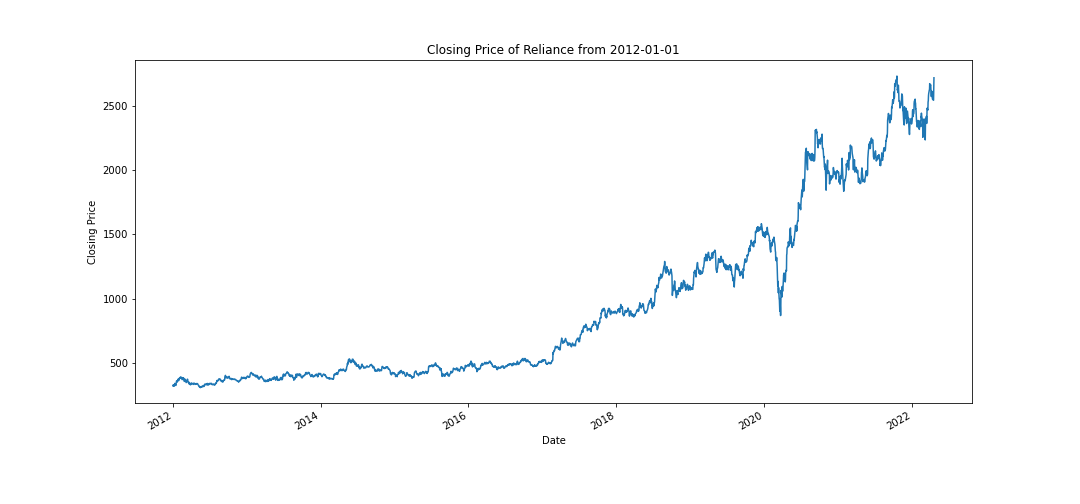
\includegraphics[scale = 0.55]{MS_Thesis_Template/figures/Rel_closing prices.png}
    \caption{ Daily closing price of Reliance stock from 2012-01-01.}
\end{figure}
Fig \ref{rel_returns} shows the daily log-returns of Reliance stock and table \ref{rel_stats} shows some statistics of the log-returns. Skewness value is positive which suggests that the log-returns are somewhat skewed to the right side rather than being symmetric . High value of kurtosis suggests that the distribution of log-returns have heavy tails which means that the tail of the log-returns distribution dies out slowly. 

\begin{figure}[H]
    \centering
    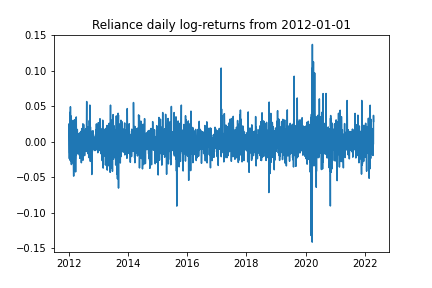
\includegraphics[scale = 0.5]{MS_Thesis_Template/figures/Rel_daily_log_returns.png}
    \caption{Daily log-returns of Reliance stock.}
    \label{rel_returns}
\end{figure}

\begin{table}[H]
\centering
\begin{tabularx}{0.7\textwidth}
{ 
  | >{\raggedright\arraybackslash}X 
  | >{\raggedright\arraybackslash}X 
  | >{\raggedright\arraybackslash}X
  | >{\raggedright\arraybackslash}X
  |}
  \hline
   Mean & Std. Dev. & Skewness & Kurtosis \\
  \hline
   0.000839 & 0.017917 & 0.076077 & 10.036623 \\
  \hline
\end{tabularx}
\caption{Some statistics of log-returns of Reliance stock.}
\label{rel_stats}
\end{table}
We first check that the log-returns series is stationary by using the Augmented Dickey-Fuller test. The null hypothesis of this statistical test is that the series is not stationary and the alternate hypothesis is that the series is stationary. Table \ref{ADF} shows that the test reports a p-value of 0 which is less than 0.05 therefore we can reject the null hypothesis and confirm the stationarity of the log-return series. 

\begin{table}[H]
\centering
\begin{tabularx}{0.7\textwidth}
{ 
  | >{\raggedright\arraybackslash}X 
  | >{\raggedright\arraybackslash}X 
  | >{\raggedright\arraybackslash}X
  |}
  \hline
    & p-value\\
   \hline
   ADF Test & 0.0\\
   
   \hline
\end{tabularx}
\caption{Augmented Dickey-Fuller test for stationarity of the log-return series.}
\label{ADF}
\end{table}

We now check that the log-return series has GARCH effects(Conditional heteroskedasticity). This is observed by the ACF(Auto Correlation function) plot of the squared log-return series which computes the correlation coefficient of the squared series with its lag-terms to check for serial correlation. Fig \ref{acf_series} shows that ACF plot has some statistically significant spikes at various lags. Blue region in the plot is the confidence interval if a spike falls in this region then it is statistically zero(no autocorrelation).
    
\begin{figure}[H]
    \centering
    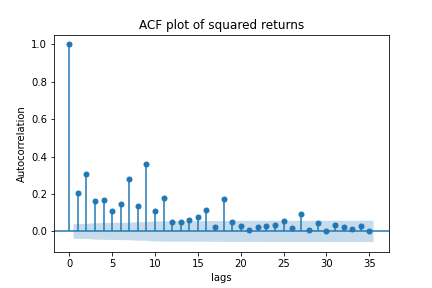
\includegraphics[scale = 0.7]{MS_Thesis_Template/figures/acf sq returns.png}
    \caption{ACF plot of the squared daily log-returns.}
\label{acf_series}    
\end{figure}
We then use the Ljung Box test to confirm for serial correlation. The null hypothesis of the test is that the series does not exhibit serial correlation and the alternate hypothesis is that it exhibits serial correlation. Table \ref{lb_series} shows the test results for first 5 lags. Since all the p-values are less than 0.05 we thus reject the null hypothesis to confirm for the presence of serial correlation.

\begin{table}[H]
\centering
\begin{tabular}{|l|*{5}{c|}}\hline
\backslashbox{L.B. test}{Lags}
&\makebox[3em]{1}&\makebox[3em]{2}&\makebox[3em]{3}
&\makebox[3em]{4}&\makebox[3em]{5}\\\hline
p-value &1.748866e-25&1.525120e-75&2.069387e-89&1.075583e-103&1.853743e-109\\\hline
\end{tabular}
\caption{Ljung-Box test for first 5 lags of the squared log-return series.}
\label{lb_series}
\end{table}
 We now use M.L.E. method as described in section \ref{garch_para_sec} to estimate the parameters of the GARCH(1,1) model using both the Gaussian and Student's t distribution innovations (noise).For convenience we will denote our model by GARCH(1,1) when Gaussian innovation is used and by t-GARCH(1,1) when Student's t distribution innovation is used. Tables \ref{garch_para} and \ref{t-garch_para} shows the estimated parameters for both the models respectively.  
\begin{table}[H]
\centering
\begin{tabularx}{0.7\textwidth}
{ 
  | >{\raggedright\arraybackslash}X 
  | >{\raggedright\arraybackslash}X 
  | >{\raggedright\arraybackslash}X
  |}
  \hline
   $\omega$ & $a$ & $b$\\
   \hline
   2.566257e-05 & 0.087744 & 0.827022\\
   
   \hline
\end{tabularx}
\caption{GARCH(1,1) estimated parameters using M.L.E.}
\label{garch_para}
\end{table}

\begin{table}[H]
\centering
\begin{tabularx}{0.7\textwidth}
{ 
  | >{\raggedright\arraybackslash}X 
  | >{\raggedright\arraybackslash}X 
  | >{\raggedright\arraybackslash}X
  | >{\raggedright\arraybackslash}X
  |}
  \hline
   $\omega$ & $a$ & $b$ & $\nu$\\
   \hline
   1.613329e-05      & 0.065359 & 0.879345  &6.083066 \\
   
   \hline
\end{tabularx}
\caption{t-GARCH(1,1) estimated parameters using M.L.E.}
\label{t-garch_para}
\end{table}

Now the conditional volatilities $\sigma_t$ can be computed using \ref{garch_sigma} for both models. Now to check the goodness of fit our models we can analyse the distributional properties of both the innovations. The series of both the innovations are computed using $\epsilon_t = \frac{r_t}{\sigma_t}$ from \ref{garch_sigma}. Fig \ref{garch_mean} shows the mean and variance of both the GARCH(1,1) and t-GARCH(1,1) innovations respectively. We observe that the mean and variance in both cases are close to 0 and 1 respectively as expected.

\begin{table}[H]
\centering
\begin{tabularx}{0.7\textwidth}
{ 
  | >{\raggedright\arraybackslash}X 
  | >{\raggedright\arraybackslash}X 
  | >{\raggedright\arraybackslash}X
  |}
  \hline
   &Mean & Variance\\
   \hline
   GARCH(1,1) innovation & 0.043317 & 0.999375\\
   \hline
   t-GARCH(1,1) innovation & 0.043671 & 1.012925\\
   \hline
\end{tabularx}
\caption{Mean and variance of the GARCH(1,1) and t-GARCH(1,1) innovations respectively.}
\label{garch_mean}
\end{table}



Now to check the distributional assumptions of our innovations the Quantile-Quantile plot (probability plot) may be used. If the distribution of the computed innovations are normal and Student's t respectively then we expect the Q-Q plot to fit straight line in both cases. From fig \ref{qq} we observe that the gaussian innovations does not fit the line properly suggesting that the distribution of the GARCH(1,1) innovation is not gaussian. Similar thing is observed for t-Garch(1,1) innovations but comparatively it fits the line better in this case.   

\begin{figure}[H]
    \centering
    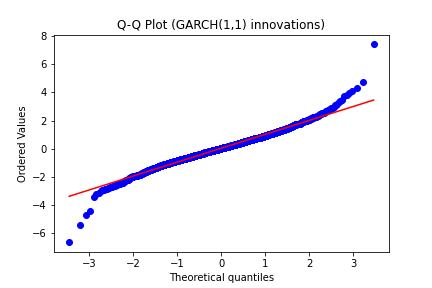
\includegraphics[scale = 0.5]{MS_Thesis_Template/figures/qq gaussian.png}
    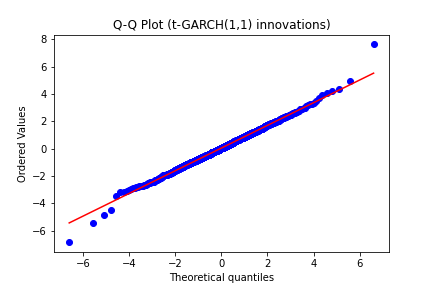
\includegraphics[scale = 0.5]{MS_Thesis_Template/figures/qq t residuals.png}
    \caption{Q-Q plots of the GARCH(1,1) and t-GARCH(1,1) innovations respectively.}
\label{qq}    
\end{figure}

We then check the normality of GARCH(1,1) innovations using Jarque–Bera and Shapiro–Wilk tests. The null hypothesis is that the series data is normally distributed and the alternate hypothesis is that the series data is not normally distributed. Table \ref{normal_test} shows that both the tests report p-values of less than 0.05. Therefore we can reject the null hypothesis and conclude that the GARCH(1,1) innovations are not normally distributed. 

\begin{table}[H]
\centering
\begin{tabularx}{0.7\textwidth}
{ 
  | >{\raggedright\arraybackslash}X 
  | >{\raggedright\arraybackslash}X 
  | >{\raggedright\arraybackslash}X
  | >{\raggedright\arraybackslash}X
  |}
  \hline
   Test  & p-value \\
   \hline
   Jarque–Bera test & 0.0 \\
   \hline
   Shapiro–Wilk test  & 4.233365e-20 \\
   
   \hline
\end{tabularx}
\caption{Normality test for the GARCH(1,1) innovations. }
\label{normal_test}
\end{table}

Table \ref{returns_stats} shows the kurtosis of empirical returns and the kurtosis implied(using \ref{gauss_kurt} and \ref{t_kurt}) by both the GARCH(1,1)  and t-GARCH(1,1) modeled returns. We observe that t-GARCH(1,1) modeled returns captures heavier tails than the GARCH(1,1) modeled returns. 

\begin{table}[H]
\centering
\begin{tabularx}{1\textwidth}
{ 
  | >{\raggedright\arraybackslash}X 
  | >{\raggedright\arraybackslash}X 
  | >{\raggedright\arraybackslash}X
  | >{\raggedright\arraybackslash}X
  |}
  \hline
    & Empirical returns &  GARCH(1,1) returns &  t-GARCH(1,1) returns \\
   \hline
   Kurtosis   & 10.036623  & 3.312534 & 7.294554\\
   
   
   \hline
\end{tabularx}
\caption{Kurtosis for empirical, GARCH(1,1) and t-GARCH(1,1) returns respectively.}
\label{returns_stats}
\end{table}
Therfore we can conclude by analysing both the innovations that the t-GARCH(1,1) model fits better to Reliance stock data as compared to the GARCH(1,1) model where Gaussian innovation is used.

\begin{figure}[H]

    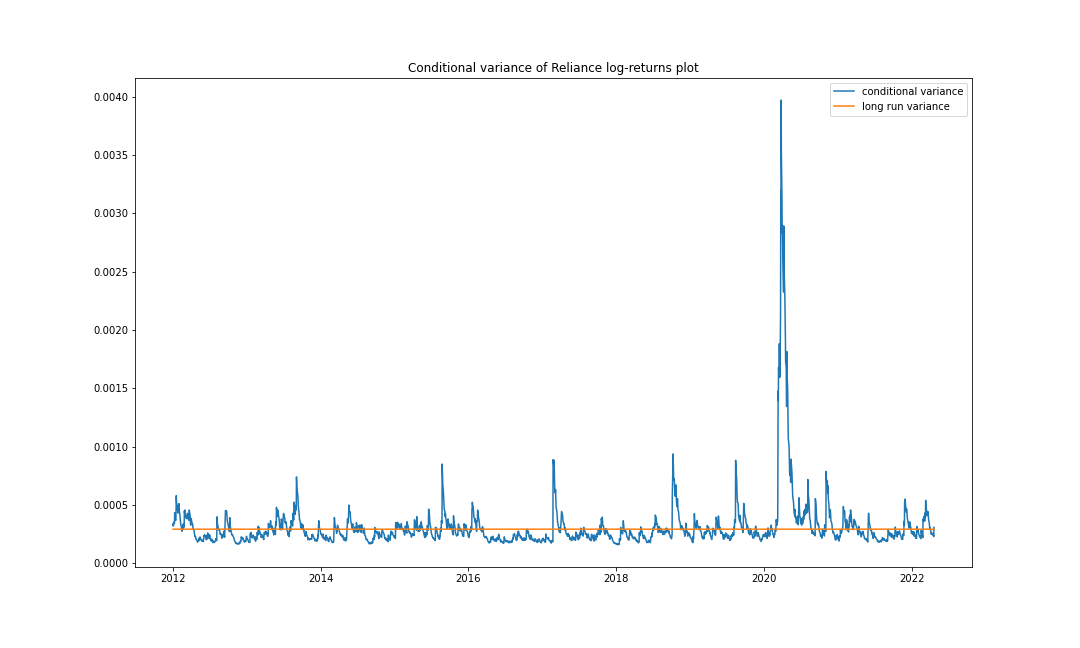
\includegraphics[scale = 0.40]{MS_Thesis_Template/figures/Cond_variance.png}
    \caption{Conditional variance computed through the 
     estimated t-GARCH(1,1) model.}
\label{cond_var}     
\end{figure}
Fig \ref{cond_var} shows the computed conditional variances ($\sigma^{2}_t$) through the estimated t-GARCH(1,1) model. It can be observed that the model captures the phenomena of volatility clustering and the mean reversion property of the conditional variances ($\sigma^{2}_t$) towards the long run variance $V_L$. The high volatile period during 2020-21 is due to the COVID-19 pandemic.

\newpage
\appendix
\definecolor{codegreen}{rgb}{0,0.6,0}
\definecolor{codegray}{rgb}{0.5,0.5,0.5}
\definecolor{codepurple}{rgb}{0.58,0,0.82}
\definecolor{backcolour}{rgb}{0.95,0.95,0.92}
 
\lstdefinestyle{mystyle}{
    backgroundcolor=\color{backcolour},   
    commentstyle=\color{violet},
    keywordstyle=\color{red},
    numberstyle=\tiny\color{cyan},
    stringstyle=\color{orange},
    basicstyle=\footnotesize,
    breakatwhitespace=false,         
    breaklines=true,                 
    captionpos=b,                    
    keepspaces=true,                 
    numbers=left,                    
    numbersep=5pt,                  
    showspaces=false,                
    showstringspaces=false,
    showtabs=false,                  
    tabsize=2
}
\lstset{style=mystyle}
\lstset{language=Python}

\chapter{Python Code used for the project}
\section{Code used for simulation of BM,Poisson,GBM,MJD and KJD paths}\label{app:appendix1}


\begin{lstlisting}
import numpy as np
import random
import matplotlib.pyplot as plt
\end{lstlisting}
\begin{lstlisting}
## BM simulation
N = 1000
BM = np.empty((N,3))
t = np.linspace(0,1,N)
for i in range(3):
    inc= np.sqrt(1/N)*np.random.normal(0,1,N-1)
    cumsum=np.cumsum(inc).tolist()
    b=[0] + cumsum
    BM[:,i] = np.array(b)
    plt.plot(t,b)
plt.title("Brownian motion paths simulation")
plt.xlabel("t")
plt.ylabel("B(t)")
plt.savefig("BM_paths")
\end{lstlisting}

\begin{lstlisting}
##GBM simulation
N = 1000
mu=0.2
sigma=0.3
t = np.linspace(0,1,N)
for i in range(3):
    s = [100]
    for j in range(N-1):
        s.append(s[j] + s[j]*mu*(1/N) + s[j]*sigma*(BM[j+1][i]-BM[j][i]))
    plt.plot(t,s) 
plt.title("GBM paths simulation") 
plt.xlabel("t")
plt.ylabel("X(t)")
plt.savefig("GBM_paths.png")
\end{lstlisting}

\begin{lstlisting}
## Poisson process generation for simulation purpose
lamda = 5
N=1000
t = np.linspace(0,1,N)
Nt = np.empty((N,3))
nt_inc = np.empty((N-1,3))
for i in range(3):
    nt_inc[:,i]=np.random.poisson(lam=lamda*(1/N),size=N-1)
    nt  = np.cumsum(nt_inc[:,i]).tolist()
    nt = [0] + nt
    Nt[:,i] = nt
plt.plot(t,Nt)    
plt.title("Poisson process paths simulation")
plt.xlabel("t")
plt.ylabel("N(t)")
plt.savefig("Poisson_simulation.png")    
\end{lstlisting}

\begin{lstlisting}
## MJD paths simulations
for i in range(3):
    sigma=0.1#diffusion voltatily
    mu=0.01#diffusion mean
    m=0 #jump mean
    delta=0.1#jump std dev
    s0=100
    diffusion=np.array([(mu - 0.5*sigma**2)*(1/N) + sigma*(BM[j+1,i]-BM[j,i]) for j in range(N-1)])
    jump =[]
    for k in nt_inc[:,i]:
        if k == 1:
            jump.append(np.random.normal(m,delta))
        else: jump.append(0) 
    jump = np.array(jump)
    r = diffusion + jump
    s = np.exp(r).tolist()
    mjd_st=[s0]
    for i in range(N-1):
        mjd_st.append(mjd_st[i]*s[i])
    plt.plot(t,mjd_st)
    plt.xlabel('t') 
    plt.ylabel('S(t)')
    plt.title('MJD paths simulation')
plt.savefig('MJD_simulation.png')
\end{lstlisting}

\begin{lstlisting}
## KJD paths simulation
for i in range(3):
    p = 0.5
    n_1 = 10
    n_2 = 10
    kou_jumps = []
    for k in nt_inc[:,i]:
        if k == 1:
            if np.random.binomial(1,p) == 1:
              kou_jumps.append(np.random.exponential(scale=1/n_1))
            else :kou_jumps.append(-np.random.exponential(scale=1/n_2))
        else: kou_jumps.append(0)
    kou_jumps = np.array(kou_jumps)
    kou_r = diffusion + kou_jumps
    kou_s = np.exp(kou_r).tolist()
    kou_st=[s0]
    for i in range(N-1):
        kou_st.append(kou_st[i]*kou_s[i])
    plt.plot(t,kou_st)
    plt.xlabel('t') 
    plt.ylabel('S(t)')
    plt.title('KJD paths simulation')
plt.savefig('KJD_simulation.png')        
\end{lstlisting}

\section{Code used for estimating BS, MJD and KJD parameters for Infosys equity}
\begin{lstlisting}
import numpy as np
import random
import matplotlib.pyplot as plt
from scipy.stats import norm
from scipy.ndimage.interpolation import shift
from numpy import prod
import pandas as pd
from matplotlib.pyplot import figure
import warnings
warnings.filterwarnings("ignore")
\end{lstlisting}

\begin{lstlisting}
def returns(data): ## compute daily simple returns
    N=len(data)
    r=np.array((N,))
    r = (data/data.shift(1))-1
    #r = r.dropna()
    r = r[1:N]
    return r
\end{lstlisting}

\begin{lstlisting}
import yfinance as yf
data = yf.download('INFY.NS',start="2014-01-01",end="2022-04-21") ##Infosys 8 years historical data
data['Adj Close'].plot(figsize = (15,7))
price = data['Adj Close']
plt.title("Closing Price of Infosys from 2014-01-01")
plt.ylabel('Closing Price')
plt.savefig('INFY_closing prices.png')
\end{lstlisting}

\begin{lstlisting}
returns_data = returns(price)
plt.plot(data.index[1:],returns_data)
plt.title("Infosys daily returns from 2014-01-01")
plt.ylabel("Daily returns")
plt.savefig('INFY_daily_returns')
\end{lstlisting}

\begin{lstlisting}
## Infosys statistics
from scipy.stats import kurtosis,skew
print(np.mean(returns_data))
print(np.var(returns_data))
print(skew(returns_data))
print(kurtosis(returns_data,fisher=False))
\end{lstlisting}

\begin{lstlisting}
## BS parameters estimation
dt = 1/252
bs_sigma = np.std(returns_data)/(dt)**0.5
bs_mu = (np.mean(returns_data) + 0.5*((bs_sigma)**2)*dt)/dt
print("BS_parameters - mu ={}, sigma ={}".format(bs_mu,bs_sigma))
\end{lstlisting}

\begin{lstlisting}
N = len(returns_data)
jumps =0
dt = 1/252
diffusion_component = []
for i in range(N): ## computing jumps
    if np.abs(returns_data[i]) >= 3*np.std(returns_data):
        jumps= jumps + 1
    else : diffusion_component.append(returns_data[i])
## initialisng parameters for MLE purpose        
initial_sigma = np.std(diffusion_component)*(1/dt)**0.5
initial_mu = (np.mean(diffusion_component) + (0.5*(initial_sigma)**2)*dt)/dt
initial_lamda = jumps*252/len(returns_data)
print(jumps)
print(3*np.std(returns_data))
print(initial_mu)
print(initial_sigma)
print(initial_lamda)
\end{lstlisting}

\begin{lstlisting}
def mjd_neg_log_likelihood(para,returns): ## computes mjd neg of log_likelihood
    x=returns
    N = len(x)
    dt = 1/252      
    mu,sigma,m,delta,lam = para
    likelihood = [] 
    for i in range(N):
        likelihood.append(lam*dt*norm.pdf(x[i],mu*dt + m,((sigma**2)*dt + delta**2)**0.5) + (1- lam*dt)*norm.pdf(x[i],mu*dt,((sigma**2)*dt)**0.5))   
    l = sum(np.log(likelihood))
    return(-l)  ## returns negative of log-likelihood

from scipy.optimize import minimize ## mjd log-likelihood optimisation for estimating parameters
bounds = ((-np.inf,np.inf),(0,np.inf),(-np.inf,np.inf),(0,np.inf),(0,np.inf)) ## bounds for estimating the parameters
mjd_res = minimize(mjd_neg_log_likelihood, (initial_mu,initial_sigma,0.5,0.5,initial_lamda),args = returns_data, method='SLSQP',bounds=bounds,options={'disp': True} )
print(mjd_res)

## MJD estimated parameters
print("MJD_parameters - mu = {},sigma = {},jump_mean = {},jump_std = {},lamda = {}".format(mjd_res.x[0],mjd_res.x[1],mjd_res.x[2],mjd_res.x[3],mjd_res.x[4]))
\end{lstlisting}

\begin{lstlisting}
def kou_neg_log_likelihood(para,returns): ## Kou neg of log_likelihood for MLE purpose
    x = returns
    N = len(x)
    dt = 1/252
    mu,sigma,lam,p,n_1,n_2 = para
    q = 1-p
    likelihood = []  
    for i in range(N):
        likelihood.append(((1-lam*dt)*norm.pdf(((x[i]-mu*dt)/(sigma*(dt)**0.5)),0,1))/(sigma*(dt)**0.5) + lam*dt*(p*n_1*np.e**((((sigma*n_1)**2)*dt*0.5) - (((x[i]-mu*dt)*n_1)))*norm.cdf(((x[i]-mu*dt-n_1*dt*(sigma)**2)/(sigma*(dt)**0.5))) + q*n_2*np.e**((((sigma*n_2)**2)*dt*0.5) + ((x[i]-mu*dt)*n_2))*norm.cdf((-(x[i]-mu*dt+n_2*dt*(sigma)**2)/(sigma*(dt)**0.5))))) 
    l = sum(np.log(likelihood))
    return(-l) ## returns negative of log-likelihood

from scipy.optimize import minimize ## kou_log-likelihood optimisation for estimating parameters
bounds = ((-np.inf,np.inf),(0,np.inf),(0,np.inf),(0,1),(1,np.inf),(0,np.inf)) ## bounds for estimating the parameters
kou_res = minimize(kou_neg_log_likelihood, (initial_mu,initial_sigma,initial_lamda,0.5,2,2),args = returns_data,bounds=bounds, method='SLSQP',options={'disp': True} )
print(kou_res)

## Kou estimated parameters
print("KJD_parameters - mu = {},sigma = {},lamda = {},p = {},n_1 = {},n_2 = {}".format(kou_res.x[0],kou_res.x[1],kou_res.x[2],kou_res.x[3],kou_res.x[4],kou_res.x[5]))
\end{lstlisting}

\begin{lstlisting}
## Simulating BS,MJD and KJD returns through estimated parameters for comparison with empirical density of returns
N = len(returns_data)
bs_sim_returns = np.random.normal(np.mean(returns_data),np.std(returns_data),N).tolist() ## BS_model simulated returns
mjd_sim_returns = []
kou_sim_returns = []
dt =1/252
mjd_mu,mjd_sigma,mjd_m,mjd_delta,mjd_lamda = mjd_res.x
kou_mu,kou_sigma,kou_lamda,p,n_1,n_2 = kou_res.x
for i in range(N):
    if np.random.binomial(1,mjd_lamda*dt) == 1: ## if there is jump for MJD_model
        mjd_sim_returns.append(mjd_mu*dt + mjd_sigma*((dt)**0.5)*np.random.normal(0,1) + np.random.normal(mjd_m,mjd_delta))
    else: mjd_sim_returns.append(mjd_mu*dt + mjd_sigma*((dt)**0.5)*np.random.normal(0,1)) ## if there is no jump for MJD_model
        
    if np.random.binomial(1,kou_lamda*dt) == 1:## if there is jump for Kou_model
        if np.random.binomial(1,p) == 1: ## positive jump for Kou_model
            kou_sim_returns.append(kou_mu*dt + kou_sigma*((dt)**0.5)*np.random.normal(0,1) + np.random.exponential(scale=1/n_1))
        ## negative jump for Kou_model
        else: kou_sim_returns.append(kou_mu*dt + kou_sigma*((dt)**0.5)*np.random.normal(0,1) - np.random.exponential(scale=1/n_2))
    
    else :  kou_sim_returns.append(kou_mu*dt + kou_sigma*((dt)**0.5)*np.random.normal(0,1))  ## if there is no jump for Kou_model       
figure(figsize=(10, 15))            
plt.subplot(3,1,1)
plt.plot(data.index[1:],returns_data)
plt.plot(data.index[1:],bs_sim_returns)
plt.legend(['Empirical returns','BS simulated returns'],loc='upper center')
plt.subplot(3,1,2)
plt.plot(data.index[1:],returns_data)
plt.plot(data.index[1:],mjd_sim_returns)
plt.legend(['Empirical returns','MJD simulated returns'],loc='upper center')
plt.subplot(3,1,3)
plt.plot(data.index[1:],returns_data)
plt.plot(data.index[1:],kou_sim_returns)
plt.legend(['Empirical returns','KJD simulated returns'],loc='upper center')
plt.savefig('simulated_returns.png')
\end{lstlisting}

\begin{lstlisting}
## Density plots
import seaborn as sns
figure(figsize=(13, 5))
sns.kdeplot(returns_data)
sns.kdeplot(bs_sim_returns)
sns.kdeplot(mjd_sim_returns)
sns.kdeplot(kou_sim_returns)
plt.xlabel('returns')
plt.legend(['Empirical returns','Black Scholes','MJD model','KJD model'])
plt.title('Kernel density plots for empirical returns and simulated returns from the models')
plt.savefig('KDE_plot_INFY.png')
\end{lstlisting}

\begin{lstlisting}
## BS statistics
dt = 1/252
bs_mean = (bs_mu - 0.5*(bs_sigma)**2)*dt
bs_std = bs_sigma*(dt)**0.5

## MJD Parameters and statistics
mu,sigma,m,delta,lamda = mjd_res.x
dt = 1/252
mjd_mean = (mu )*dt + m*lamda*dt
mjd_variance = (sigma**2)*dt + ((lamda*dt))*(delta**2 + m**2)
mjd_skewness = ((3*delta**2 + m**2)*m*lamda*dt)/mjd_variance**(3/2)
mjd_kurtosis = ((3*(delta)**4 + 6*(m*delta)**2 + (m)**4)*lamda*dt)/(mjd_variance)**2 + 3

## Kou Parameters and statistics
mu,sigma,lamda,p,n_1,n_2 = kou_res.x
q =1-p
kou_mean = mu*dt + lamda*((p/n_1)-(q/n_2))*dt
kou_variance = (sigma**2)*dt + (p*q*((1/n_1 + 1/n_2))**2 + (p/(n_1)**2 + q/(n_2)**2 ))*lamda*dt + lamda*dt*(p/n_1 - q/n_2)**2
kou_skewness =  6*(p/n_1**3 - q/n_2**3)*lamda*dt/(kou_variance)**(3/2)
kou_kurtosis = (24*(p/(n_1)**4 + q/(n_2)**4)*lamda*dt)/(kou_variance)**2 + 3
\end{lstlisting}
 
\section{Code used for pricing Infosys call options under BS, MJD and KJD models respectively}
\begin{lstlisting}
import numpy as np
import random
from scipy.stats import norm
import pandas as pd
\end{lstlisting}
\begin{lstlisting}
def BS_call(S0,K,T,r,sigma): ## calculate BS call price
    T=T/365
    d1 = (np.log(S0/K) + (r+0.5*(sigma)**2)*T)/(sigma*np.sqrt(T))
    d2 = (np.log(S0/K) + (r-0.5*(sigma)**2)*T)/(sigma*np.sqrt(T))
    call_price = S0*norm.cdf(d1) - (K*np.exp(-r*T)*norm.cdf(d2))
    return round(call_price,5)

## MJD option price calculation (Monte Carlo method)
def mjd_price_call(para,r,T,S0,Strike):
    T = T/365
    sigma,m,delta,lamda = para
    k = (np.e**(m + ((delta)**2)*0.5)) - 1
    sim = 100000
    b_T = np.random.normal(0,1,sim)*(T)**0.5
    n_T = np.random.poisson(lam=lamda*(T),size=sim)
    jumps_component = np.array([np.sum(np.random.normal(m, delta,n_T[i])) for i in range(sim)])
    s_T = S0*np.e**((r-0.5*(sigma)**2-lamda*k)*T + sigma*b_T + jumps_component)
    discounted_payoff = []
    for i in range(sim):
        discounted_payoff.append(np.e**((-r)*T)*(max(s_T[i]-Strike,0)))
    return round(np.mean(discounted_payoff),5) 

## Kou model option price calculation (Monte Carlo method)
def kou_price_call(para,r,T,S0,Strike):
    T = T/365
    sigma,lamda,p,n_1,n_2 = para
    k= (p*n_1)/(n_1 -1) + (q*n_2)/(n_2 + 1) - 1
    sim = 100000
    b_T = np.random.normal(0,1,sim)*(T)**0.5
    n_T = np.random.poisson(lam=lamda*(T),size=sim)
    jumps = []
    for i in range(sim):
        temp =[] ##list for storing jump points
        for j in range(n_T[i]):
            if np.random.binomial(1,p) == 1:
                temp.append(np.random.exponential(scale=1/n_1))
            else : temp.append(-np.random.exponential(scale=1/n_2))
        jumps.append(sum(temp))
    jumps_component = np.array(jumps)    
    s_T = S0*np.e**((r-0.5*(sigma)**2-lamda*k)*T + sigma*b_T + jumps_component)
    discounted_payoff = []
    for i in range(sim):
        discounted_payoff.append(np.e**((-r)*T)*(max(s_T[i]-Strike,0)))
    return round(np.mean(discounted_payoff),5) 
           
\end{lstlisting}

\begin{lstlisting}
Pricing Infosys Call options dated 21/04/22, S0 =1615.70 ,expiry-26/05/22

call_data = pd.read_csv('infy21april.csv')
call_data["ASK PRICE"] = [float(str(i).replace(",", "")) for i in call_data["ASK PRICE"]]
call_data["STRIKE PRICE"] = [float(str(i).replace(",", "")) for i in call_data["STRIKE PRICE"]]
call_data

df = call_data
K = [df['STRIKE PRICE'][i] for i in range(len(df))]
BS_prices = []
MJD_prices = []
Kou_prices = []
mid_prices = (call_data["ASK PRICE"] + call_data["BID PRICE"])/2
for i in range(len(df)):
    BS_prices.append(BS_call(S0=1615.70,K=K[i],T=35,r=0.045,sigma=np.std(returns_data)*(252)**0.5))
    MJD_prices.append(mjd_price_call(mjd_res.x[1:5],r=0.045,T=35,S0=1615.70,Strike=K[i]))
    Kou_prices.append(kou_price_call(kou_res.x[1:6],r=0.045,T=35,S0=11615.70,Strike=K[i]))

Prices = pd.DataFrame({'STRIKE PRICE':K,'BID PRICE':df['BID PRICE'],'ASK PRICE':df['ASK PRICE'],'MID PRICE':mid_prices,
                       'BS PRICE':BS_prices,'MJD PRICE':MJD_prices,'KJD PRICE':Kou_prices})
Prices ## Computed prices     
\end{lstlisting}

\section{Code used for computing implied volatilities for TATA MOTORS stock and NIFTY50 stock index data respectively}
\begin{lstlisting}
import numpy as np
import random
import pandas as pd
from scipy.stats import norm
import matplotlib.pyplot as plt
import warnings
\end{lstlisting}

\begin{lstlisting}
def BS_call(S0,K,T,r,sigma): ## calculate BS call price
    T=T/365
    d1 = (np.log(S0/K) + (r+0.5*(sigma)**2)*T)/(sigma*np.sqrt(T))
    d2 = (np.log(S0/K) + (r-0.5*(sigma)**2)*T)/(sigma*np.sqrt(T))
    call_price = S0*norm.cdf(d1) - (K*np.exp(-r*T)*norm.cdf(d2))
    return call_price
def vega_call(S0,K,T,r,sigma):# vega will be used in Newton-Raphson method
    T=T/365
    d1 = (np.log(S0/K) + (r+0.5*(sigma)**2)*T)/(sigma*np.sqrt(T))
    vega = S0*norm.pdf(d1,0,1)*(T)**(0.5)
    return vega
\end{lstlisting}

\begin{lstlisting}
def imp_vol(price_data,S0,T,r): ## computes implied volatility
    data = price_data
    ## price_data preprocessing
    if 'ASK PRICE' in data.columns:
        data["ASK PRICE"] = [float(str(i).replace(",", "")) for i in data["ASK PRICE"]]# removing comas from data entries if found to convert them in float
        data["BID PRICE"] = [float(str(i).replace(",", "")) for i in data["BID PRICE"]]
        data["STRIKE PRICE"] = [float(str(i).replace(",", "")) for i in data["STRIKE PRICE"]]
        price = data[['ASK PRICE', 'BID PRICE']].mean(axis=1) ##Market price that will be used
    elif 'Settle Price' in data.columns:
        data = data.rename(columns={'Strike Price':'STRIKE PRICE'})
        price = data['Settle Price']
    else: warnings.warn("No price data found")
    temp = np.linspace(0,1,1000)    
    vol = [] # to store imp vol 
    u=1 #right most point of interval
    l=0 #left most point of interval 
# Finding the interval of convergence for Newton-Raphson method
    for i in range(len(price)):
        K=data['STRIKE PRICE'][i]
        for j in range(1,len(temp)):
            if BS_call(S0,K,T,r,temp[j]) > price[i]:
                l = temp[j-1]
                break
        for k in range(1,len(temp)):    
            if BS_call(S0,K,T,r,temp[-(k+1)]) < price[i]:   
                u = temp[-k]
                break
        g = random.uniform(l,u)## initial point for Newton-Raphson method
        h = (BS_call(S0,K,T,r,g) - price[i])/(vega_call(S0,K,T,r,g))
        while abs(h) > 0.001:
            g = g - h
            h = (BS_call(S0,K,T,r,g) - price[i])/(vega_call(S0,K,T,r,g))  
        vol.append(round(g,4))
    return(np.array(vol))
\end{lstlisting}

\begin{lstlisting}
Computing TATA Motors call options implied volatility
## TATA_Motors,Dated-28/01/2022,S0=497.30,T=27
tata_data = pd.read_csv('tata.csv')

tata_iv = imp_vol(tata_data,S0=497.30,T=27,r=0.1)
MID_PRICE = (tata_data["BID PRICE"] + tata_data["ASK PRICE"])/2
plt.plot(tata_data['STRIKE PRICE'],tata_iv,'o')
iv_list = tata_data['IV'].tolist()
IV = [i*0.01 for i in iv_list]
rmse = np.sqrt(np.sum((np.array(IV) - np.array(tata_iv))**2)/len(IV))
plt.plot(tata_data['STRIKE PRICE'],IV,'*')
plt.legend(loc="upper right") 
plt.legend(["Calculated I.V.","NSE Option Chain Site I.V."])
plt.xlabel('Strike Price')
plt.ylabel('Implied Volatility')
plt.title("TATA MOTORS Call Options Implied volatility plot ")
plt.savefig("TATA_IV_plot.png")
print(rmse)
\end{lstlisting}

\begin{lstlisting}
Computing NIFTY50 call options implied volatility,S0=17053.95,dated 29/11/2021 
data1 =pd.read_csv('nifty_29nov_2dec.csv')
data1=data1[(data1['Strike Price'].between(16800,18200))&(data1['Date'] == '29-Nov-2021' )].reset_index()
data2 =pd.read_csv('nifty_29nov_9dec.csv')
data2=data2[(data2['Strike Price'].between(16800,18200))&(data2['Date'] == '29-Nov-2021' )].reset_index()
data3 =pd.read_csv('nifty_29nov_16dec.csv')
data3=data3[(data3['Strike Price'].between(16800,18200))&(data3['Date'] == '29-Nov-2021' )].reset_index()
data4 =pd.read_csv('nifty_29nov_30dec.csv')
data4=data4[(data4['Strike Price'].between(16800,18200))&(data4['Date'] == '29-Nov-2021' )]
data4 = data4.sort_values(by=['Strike Price'], ascending=True)
data4 = data4.reset_index()
d1=imp_vol(data1,S0=17053.95,T=3,r=0.1)
d2=imp_vol(data2,S0=17053.95,T=10,r=0.1)
d3=imp_vol(data3,S0=17053.95,T=17,r=0.1)
d4=imp_vol(data4,S0=17053.95,T=31,r=0.1)
plt.plot(data1['Strike Price'],d1,'o',label = 'T=3 days')
plt.plot(data2['Strike Price'],d2,'o',label = 'T=10 days')
plt.plot(data3['Strike Price'],d3,'o',label = 'T=17 days')
plt.plot(data4['Strike Price'],d4,'o',label = 'T=31 days')
plt.legend(loc="upper center") 
plt.xlabel('Strike Price')
plt.ylabel('Implied Volatility')
plt.title("NIFTY50 Call Options Implied volatility with different maturities ")
plt.savefig("NIFTY50_IV_plot.png")

## plotting NIFTY50 volatility surface
x1 =np.zeros((len(data1),4))
for i in range(len(data1)):
    x1[i][0]=d1[i]
for i in range(len(data1)):
    x1[i][1]=d2[i]
for i in range(len(data1)):
    x1[i][2]=d3[i]
for i in range(len(data1)):
    x1[i][3]=d4[i]    
y1 = np.zeros((len(data1),4))
for j in range(4):
    for i in range(len(data1)):
        y1[i][j]=data1['Strike Price'][i]
z1 = np.zeros((len(data1),4))
l=[3,10,17,31]
for j in range(4):
    for i in range(len(data1)):
        z1[i][j]=l[j]   
from mpl_toolkits.mplot3d import Axes3D
from matplotlib import pyplot as plt
from matplotlib.pyplot import figure
figure(figsize=(13, 10))
fig = plt.figure()
ax = Axes3D(fig,auto_add_to_figure=False)
ax.plot_surface(y1,z1,x1,cmap='Reds',edgecolor='black')
ax.invert_xaxis()
ax.set_ylabel('Maturities(days)')
ax.set_xlabel('Strike Price')
ax.set_zlabel('I.V.')
fig.add_axes(ax)
#ax.set_zlim(0.20,0.45)
ax.view_init(30,30)
plt.title('NIFTY50 Call Options volatility surface')
plt.show()
\end{lstlisting}

\section{Code used for estimating the GARCH(1,1) model parameters for Reliance equity}

\begin{lstlisting}
import numpy as np
import random
import matplotlib.pyplot as plt
import pandas as pd
from matplotlib.pyplot import figure
from scipy.ndimage.interpolation import shift
import warnings
warnings.filterwarnings("ignore")
\end{lstlisting}

\begin{lstlisting}
def returns(data): ## compute daily log returns
    N=len(data)
    #r=np.array((N,))
    r = np.log(data) - np.log(data.shift(1))
    #r = r.dropna()
    r = r[1:N]
    return r

import yfinance as yf
data = yf.download('RELIANCE.NS',start="2012-01-01",end="2022-03-31") ##Reliance 10 years historical data
data['Adj Close'].plot(figsize = (15,7))
plt.title("Closing Price of Reliance from 2012-01-01")
plt.ylabel('Closing Price')
plt.savefig('Rel_closing prices.png')
price = data['Adj Close']

returns_data = returns(price)
plt.plot(data.index[1:],returns_data)
plt.title('Reliance daily log-returns from 31/03/2012')
plt.savefig('Rel_daily_log_returns')
\end{lstlisting}

\begin{lstlisting}
## Reliance statistics
from scipy.stats import kurtosis,skew
print(np.mean(returns_data))
print(np.std(returns_data))
print(skew(returns_data))
print(kurtosis(returns_data,fisher=False))
\end{lstlisting}

\begin{lstlisting}
from statsmodels.tsa.stattools import adfuller
res = adfuller(returns_data)
print('Augmneted Dickey_fuller Statistic: %f' % res[0])
print('p-value: %f' % res[1])
\end{lstlisting}

\begin{lstlisting}
from statsmodels.graphics.tsaplots import plot_pacf,plot_acf
plot_acf((returns_data**2))## checking for correlation
plt.xlabel('lags')
plt.ylabel('Autocorrelation')
plt.title('ACF plot of squared returns')
plt.show()

from statsmodels.stats.diagnostic import acorr_ljungbox
acorr_ljungbox(returns_data**2,lags=5, return_df=True)
\end{lstlisting}

\begin{lstlisting}
def Garch(para,returns): ## compute the volatilities, input parameters = (omega,a,b) 
    N = len(returns)
    omega,a,b = para[0:3]  ## cond_mean = 0(assumption)
    cond_variance = np.zeros((N,))  ##array to store the volatilities
    #long_run_variance = omega/(1-a-b)
    cond_variance[0] = np.std(returns)**2 ## initialising cond_variance
    #cond_variance[0] = long_run_variance ## initialising cond_variance
    for i in range(1,N):
        cond_variance[i] = omega + a*(returns[i-1])**2 + b*(cond_variance[i-1])    
    return cond_variance ## sigma_squared values
    
from scipy.special import gamma
def neg_log_likelihood(para,returns,noise): ## computes negative of log-likelihood which will be minimized using scipy.optimise.minimise  
    N= len(returns)                   ## for estimating the parameters.
    cond_variance = Garch(para,returns)
    if noise == 'normal':
        ll = -0.5*sum([np.log(2*(np.pi)) + np.log(cond_variance[j]) + returns[j]**2/cond_variance[j] for j in range(N)])
    elif noise == 't':
        nu = para[3]
        c = np.log([gamma((nu+1)/2)/(gamma(nu/2)*(np.pi*(nu-2))**0.5)])
        ll = c*N - sum([np.log((cond_variance[j])**0.5) for j in range(N)]) - ((nu+1)/2)*sum([np.log(1+(returns[j]**2/((nu-2)*(cond_variance[j])))) for j in range(N)])
    return (-ll)
\end{lstlisting}

\begin{lstlisting}
Taking the noise as Gaussian

from scipy.optimize import minimize
bounds = ((0.0001,None),(0.0001,0.9999),(0.0001,0.9999)) ## bounds for estimating the parameters
res_gauss = minimize(neg_log_likelihood, (0.1,0.05,0.9),args =(np.array(returns_data)*100,'normal'), method='SLSQP',options={'disp': True})
print(res_gauss)
omega,a,b = res_gauss.x

omega = omega/10000 ## For optimisation purpose the returns were converted into percentage and thus the estimate of omega was scaled by 10000.
print("Estimated parameters : omega={}, a={}, b={}".format(omega,a,b))

Gaussian Noise Analysis

cond_variance = Garch((omega,a,b),returns_data)
noise_gauss = np.array(returns_data)/np.sqrt(cond_variance)
print(np.mean(noise_gauss))
print(np.var(noise_gauss))

from scipy import stats
stats.probplot(noise_gauss,dist = stats.norm,plot=plt)
plt.title("Q-Q Plot (GARCH(1,1) innovations)")

from scipy.stats import jarque_bera,shapiro
print(jarque_bera(noise_gauss))
print(shapiro(noise_gauss))
\end{lstlisting}

\begin{lstlisting}
Taking noise from "Student's t distribution"

from scipy.optimize import minimize
bounds = ((0.0001,None),(0.0001,0.9999),(0.0001,0.9999)) ## bounds for estimating the parameters
res_t = minimize(neg_log_likelihood, (0.1,0.05,0.9,6),args =(np.array(returns_data)*100,'t'), method='SLSQP',options={'disp': True})
print(res_t)
omega_t,a_t,b_t,nu_t = res_t.x

omega_t = omega_t/10000 ## For optimisation purpose the returns were converted into percentage and thus the estimate of omega was scaled by 10000.
print("Estimated parameters : omega={}, a={}, b={}, nu={}".format(omega_t,a_t,b_t,nu_t))

Noise analysis t-GARCH(1,1) estimated model

cond_variance_t = Garch((omega_t,a_t,b_t,nu_t),np.array(returns_data))
noise_t = np.array(returns_data)/np.sqrt(cond_variance_t)
print(np.mean(noise_t))
print(np.var(noise_t))

from scipy import stats
stats.probplot(noise_t,dist = stats.t(df=nu_t),plot=plt)
plt.title("Q-Q Plot (t-GARCH(1,1) innovations)")
plt.show()

## Implied  Kurtosis from both innovations of GARCH(1,1) model
gauss_kurtosis = 3*(1-(a+b)**2)/(1-2*(a**2) - (a+b)**2)
t_kurtosis = (6/(nu_t-4) + 3)*(1-(a_t+b_t)**2)/(1-2*(a_t**2) - (a_t+b_t)**2 - 6*((a_t)**2)/(nu_t-4))
print(gauss_kurtosis)
print(t_kurtosis)

## From the Q-Q plot and kurtosis values we see that Student's t distribution performs well as compared to normal distribution for noise. 

omega,a,b = res_t.x[0:3] ## estimated parameters of t-GARCH(1,1) model
long_term_variance = omega_t/((1-a_t-b_t))
figure(figsize=(15, 9))
plt.plot(data.index[1:],cond_variance_t)## cond_volatility plot with the std. residuals as Student's t distribution
plt.plot(data.index[1:],np.array([long_term_variance for i in range(len(data.index[1:]))]))
plt.legend(['conditional variance','long run variance'])
plt.title('Conditional variance of Reliance log-returns plot')
plt.savefig("Cond_variance.png")
\end{lstlisting}

\chapter{Computed Implied Volatilities of Call options for TATA MOTORS stock  and NIFTY50 stock index data respectively}\label{app:appendix2}

\begin{table}[H]
\centering
\tiny
\begin{tabularx}{1.1\textwidth}
  { 
  | >{\raggedright\arraybackslash}X 
  | >{\raggedright\arraybackslash}X 
  | >{\raggedright\arraybackslash}X 
  | >{\raggedright\arraybackslash}X
  | >{\raggedright\arraybackslash}X 
  | >{\raggedright\arraybackslash}X 
  |}
  \hline
   BID PRICE & ASK PRICE & MID PRICE & STRIKE PRICE & I.V.(NSE Site) & I.V.(computed) \\
   \hline   
   54.95     & 56.1      & 55.525    & 460          & 0.6186         & 0.5998         \\
   \hline
   47.6      & 48.1      & 47.85     & 470          & 0.5834         & 0.5739         \\
   \hline
   40.5      & 40.9      & 40.7      & 480          & 0.5659         & 0.5509         \\
   \hline
   34.2      & 34.4      & 34.3      & 490          & 0.5334         & 0.5347         \\
   \hline
   28.6      & 28.7      & 28.65     & 500          & 0.5232         & 0.5227         \\
   \hline
   23.75     & 23.9      & 23.825    & 510          & 0.516          & 0.5158         \\
   \hline
   19.4      & 19.5      & 19.45     & 520          & 0.5088         & 0.5068         \\
   \hline
   15.65     & 15.8      & 15.725    & 530          & 0.5027         & 0.5012         \\
   \hline
   12.65     & 12.8      & 12.725    & 540          & 0.5005         & 0.4989         \\
   \hline
   10.1      & 10.2      & 10.15     & 550          & 0.497          & 0.4964         \\
   \hline
   8.1       & 8.2       & 8.15      & 560          & 0.4965         & 0.4961         \\
   \hline
   6.5       & 6.55      & 6.525     & 570          & 0.4987         & 0.4977         \\
   \hline
   5.25      & 5.35      & 5.3       & 580          & 0.5028         & 0.5027         \\
   \hline
   .3       & 4.4       & 4.35      & 590          & 0.5093         & 0.5092         \\
   \hline
   3.6       & 3.7       & 3.65      & 600          & 0.5207         & 0.5193         \\
   \hline
   2.9       & 3         & 2.95      & 610          & 0.5272         & 0.5227         \\
   \hline
   2.4       & 2.5       & 2.45      & 620          & 0.5302         & 0.5304         \\
   \hline
   2         & 2.05      & 2.025     & 630          & 0.5382         & 0.5371\\
   \hline
\end{tabularx}
 \caption{Computed I.V. values using Newton-Raphson method and the I.V. values listed on NSE option chain site of TATA MOTORS stock call options. }
\end{table}

\begin{table}[H]
\centering
\tiny
\begin{tabularx}{1.1\textwidth}
{ 
  | >{\raggedright\arraybackslash}X 
  | >{\raggedright\arraybackslash}X 
  | >{\raggedright\arraybackslash}X 
  | >{\raggedright\arraybackslash}X
  | >{\raggedright\arraybackslash}X
  | >{\raggedright\arraybackslash}X
  | >{\raggedright\arraybackslash}X
  | >{\raggedright\arraybackslash}X
  | >{\raggedright\arraybackslash}X
  |}
  \hline
   STRIKE PRICE & Settle Price(T=3) & I.V.(T=3) & Settle Price(T=10) & I.V.(T=10) & Settle Price(T=17) & I.V.(T=17) & Settle Price(T=31) & I.V.(T=31) \\
   \hline
   16800        & 330.45            & 0.2657    & 408.7              & 0.2045     & 455.45             & 0.1754     & 525.7              & 0.1459     \\
   \hline
   16850        & 289.9             & 0.2567    & 371.1             & 0.2002     & 425.05           & 0.1783     & 490.0            & 0.1451     \\
   \hline
   16900        & 249.9             & 0.2472    & 335.7              & 0.1981     & 382.35             & 0.1702     & 458.25             & 0.1453     \\
   \hline
   16950        & 212.95            & 0.2389    & 300.35             & 0.1934     & 393.9              & 0.2005     & 424.85             & 0.1442     \\
   \hline
   17000        & 179.3             & 0.2317    & 268.25             & 0.1904     & 324.75             & 0.1727     & 390.7              & 0.1429     \\
   \hline
   17050        & 147.3             & 0.2233    & 236.6              & 0.1866     & 291.6              & 0.17       & 362.75             & 0.1425     \\
   \hline
   17100        & 119.7             & 0.2191    & 208.35             & 0.1847     & 265.6              & 0.1701     & 333.2              & 0.1422     \\
   \hline
   17150        & 94.25             & 0.2121    & 180.6              & 0.181      & 231.4              & 0.163      & 304.7              & 0.1421     \\
   \hline
   17200        & 72.2              & 0.2061    & 155.25             & 0.1776     & 208.85             & 0.164      & 278.7              & 0.1402     \\
   \hline
   17250        & 53.85             & 0.2002    & 132.45             & 0.1746     & 187.15             & 0.1636     & 252.85             & 0.1393     \\
   \hline
   17300        & 38.65             & 0.1946    & 111.8              & 0.1731     & 162.95             & 0.1602     & 230.15             & 0.1396     \\
   \hline
   17350        & 27.6              & 0.1919    & 93.15              & 0.1702     & 143.0              & 0.16       & 208.4              & 0.1383     \\
   \hline
   17400        & 19.4              & 0.1899    & 76.25              & 0.1667     & 122.95             & 0.1568     & 187.45             & 0.1382     \\
   \hline
   17450        & 13.5              & 0.1886    & 62.05              & 0.1646     & 107.05             & 0.1552     & 168.0              & 0.1377     \\
   \hline
   17500        & 9.5               & 0.1892    & 49.65              & 0.1621     & 90.0               & 0.1536     & 151.3              & 0.1371     \\
   \hline
   17550        & 6.65              & 0.1893    & 39.4               & 0.1599     & 75.85              & 0.1519     & 134.45             & 0.1368     \\
   \hline
   17600        & 4.8               & 0.1927    & 30.7               & 0.1572     & 63.85              & 0.1494     & 119.5              & 0.1364     \\
   \hline
   17650        & 3.85              & 0.1992    & 24.05              & 0.1568     & 57.15              & 0.1526     & 105.5              & 0.1357     \\
   \hline
   17700        & 3.2               & 0.2066    & 18.6               & 0.1556     & 44.6               & 0.1473     & 92.9               & 0.1355     \\
   \hline
   17750        & 2.75              & 0.2151    & 15.05              & 0.1568     & 39.2               & 0.1498     & 81.85              & 0.1348     \\
   \hline
   17800        & 2.5               & 0.2233    & 12.35              & 0.1575     & 30.65              & 0.1463     & 71.35              & 0.1344     \\
   \hline
   17850        & 2.4               & 0.2343    & 10.5               & 0.1608     & 80.35              & 0.2117     & 62.5               & 0.1349     \\
   \hline
   17900        & 2.25              & 0.2457    & 8.8                & 0.1633     & 21.9               & 0.1487     & 54.6               & 0.1341     \\
   \hline
   17950        & 2.1               & 0.2551    & 7.65               & 0.1667     & 25.7               & 0.1614     & 48.2               & 0.1344     \\
   \hline
   18000        & 1.95              & 0.2649    & 7.2                & 0.1722     & 16.5               & 0.1512     & 42.6               & 0.1361     \\
   \hline
   18050        & 1.75              & 0.2729    & 6.35               & 0.1757     & 13.9               & 0.1523     & 36.75              & 0.1358     \\
   \hline
   18100        & 1.6               & 0.2805    & 5.8                & 0.1809     & 12.7               & 0.1554     & 31.35              & 0.1343     \\
   \hline
   18150        & 1.55              & 0.2906    & 5.3                & 0.1844     & 13.7               & 0.1645     & 27.45              & 0.1353     \\
   \hline
   18200        & 1.45              & 0.2997    & 5.05               & 0.1908     & 10.35              & 0.1617     & 23.75              & 0.1353\\  
   \hline
\end{tabularx}
\caption{Computed I.V. values of call options of NIFTY50 stock index with different maturities.}
\end{table}

%%%
% This code snippet takes care of the required  
% Equation/Figure numbering scheme.
\renewcommand\thefigure{\thechapter.\arabic{figure}}    
\renewcommand{\theequation}{\thechapter.\arabic{equation}}
\setcounter{equation}{0}
\setcounter{figure}{0}
%%%



\clearpage

\newpage

% Use the relevant bibliography style file.
% Mathematics: amsalpha.bst
% Physics: these.bst
% Chemistry: achemso.bst (or) biochem.bst 
\bibliographystyle{alpha}
\bibliography{Bibliography}


\end{document}












